\documentclass[../main]{subfiles}

\questiontrue
\solutiontrue

\begin{document}
    \ifquestion
    
	\section{Apollo XXVI}

\parte{A}{''Optical'' Rocket}

Consider a converging lens with radius $R$ and focal ratio $\beta$ in the vacuum of space. A celestial object illuminates the lens, which is perpendicular to the direction of light propagation. The radiation flux in that region of space is $F_\odot$. The lens has mass $m$. The object is far enough that the flux remains practically constant with distance.

\ut{A.1} Neglecting relativistic effects, determine the thrust force of the lens.

\ut{A.2} The Hubble telescope, with mass $m = 11\,110 \text{ kg}$, has a primary lens with $\beta = 24$ and diameter $D = 2.4 \text{ m}$. Determine how long it would take for it to travel a distance equal to the Earth's diameter (neglecting the gravitational attraction of the Earth and Sun).

\ut{A.3} What should be the mass of a star with the same luminosity as the Sun for the telescope to remain stationary in space?

\parte{B}{Matter Cannon}

Consider a rocket with initial mass $m_0$ that ejects propellant at speed $u$ relative to its engines and starts from rest at $t = 0$. The rocket's mass can be described by the relation $m(t) = m_0 f(t)$.

\ut{B.1} Considering relativistic effects, find the relation for the rocket’s velocity as a function of time.

\ut{B.2} Approximate the expression for non-relativistic cases and show that the equation becomes:

$$V(t) = -u \ln(f(t))$$

\parte{C}{Radiation Cannon}

Consider a rocket with initial mass $m_0$ that ejects radiation as propulsion, starting from rest at $t = 0$. The rocket's mass can be described by $m(t) = m_0 f(t)$. Considering relativistic effects, find the relation for the rocket's velocity as a function of time.

\parte{D}{Ion Propulsion}

Sapphire, a researcher from the planet Pluto II, contributed greatly to the development and improvement of rocket propulsion techniques and science on her world. In the year 3170, she developed a new liquid fuel for combustion engines, and later, in 3173, she created a design for engines powered by ions accelerated by potentials.

Regarding this last propulsion method, consider the scheme in Figure \ref{fig:motor}.

	\begin{figure}[htpb]
	\centering
		
		\tikzset{every picture/.style={line width=0.75pt}} %set default line width to 0.75pt        
		
		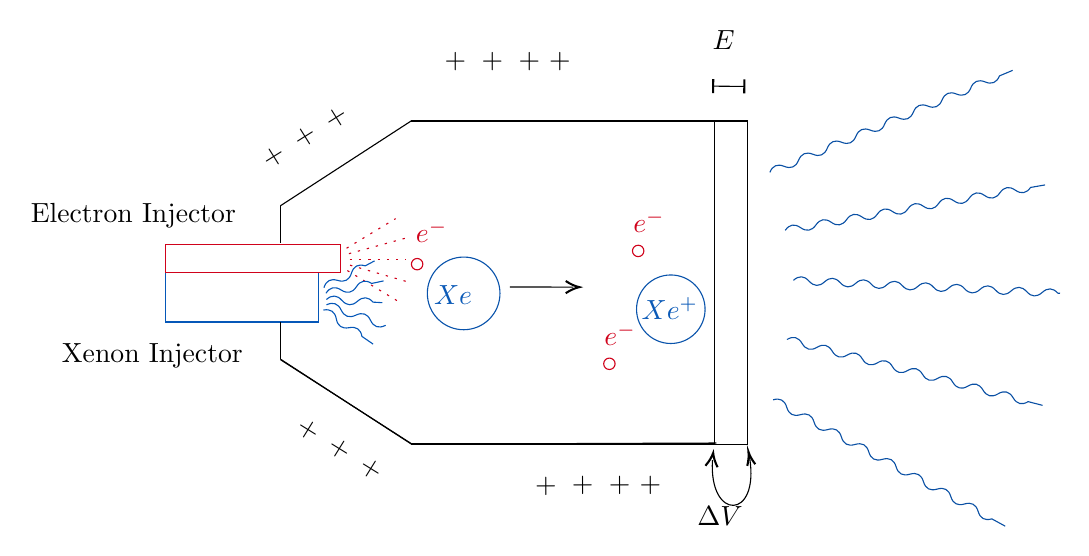
\begin{tikzpicture}[x=0.75pt,y=0.75pt,yscale=-1.5,xscale=1.5]
			%uncomment if require: \path (0,436); %set diagram left start at 0, and has height of 436
			
			%Shape: Rectangle [id:dp6321961395514091] 
			\draw  [color={rgb, 255:red, 5; green, 87; blue, 184 }  ,draw opacity=1 ] (204.19,210.05) -- (253.33,210.05) -- (253.33,225.83) -- (204.19,225.83) -- cycle ;
			%Shape: Rectangle [id:dp44586851776757674] 
			\draw  [color={rgb, 255:red, 208; green, 2; blue, 27 }  ,draw opacity=1 ] (204.19,200.83) -- (260.19,200.83) -- (260.19,210.05) -- (204.19,210.05) -- cycle ;
			%Shape: Rectangle [id:dp0031641197361298445] 
			\draw   (380.43,161.25) -- (391,161.25) -- (391,265.17) -- (380.43,265.17) -- cycle ;
			%Straight Lines [id:da18083554258725254] 
			\draw    (283,161.25) -- (241,188.5) ;
			%Straight Lines [id:da9904337451299869] 
			\draw    (241,188.5) -- (241,200.5) ;
			%Straight Lines [id:da2580970056544176] 
			\draw    (241,225.92) -- (241,237.75) ;
			%Straight Lines [id:da2763631057614282] 
			\draw    (283,265) -- (241,237.75) ;
			%Straight Lines [id:da3962273381232304] 
			\draw    (283,161.25) -- (380.43,161.25) ;
			%Straight Lines [id:da7529974710766334] 
			\draw    (283,265) -- (380.43,265) ;
			%Shape: Circle [id:dp47285000676239086] 
			\draw  [color={rgb, 255:red, 9; green, 83; blue, 171 }  ,draw opacity=1 ] (288.19,216.64) .. controls (288.19,210.2) and (293.41,204.97) .. (299.86,204.97) .. controls (306.3,204.97) and (311.52,210.2) .. (311.52,216.64) .. controls (311.52,223.08) and (306.3,228.31) .. (299.86,228.31) .. controls (293.41,228.31) and (288.19,223.08) .. (288.19,216.64) -- cycle ;
			%Shape: Circle [id:dp5936031056054498] 
			\draw  [color={rgb, 255:red, 208; green, 2; blue, 27 }  ,draw opacity=1 ] (286.75,207.25) .. controls (286.75,206.24) and (285.93,205.42) .. (284.92,205.42) .. controls (283.9,205.42) and (283.08,206.24) .. (283.08,207.25) .. controls (283.08,208.26) and (283.9,209.08) .. (284.92,209.08) .. controls (285.93,209.08) and (286.75,208.26) .. (286.75,207.25) -- cycle ;
			%Straight Lines [id:da12111598442422489] 
			\draw    (314.72,214.57) -- (335,214.62) ;
			\draw [shift={(337,214.63)}, rotate = 180.13] [color={rgb, 255:red, 0; green, 0; blue, 0 }  ][line width=0.75]    (4.37,-1.96) .. controls (2.78,-0.92) and (1.32,-0.27) .. (0,0) .. controls (1.32,0.27) and (2.78,0.92) .. (4.37,1.96)   ;
			%Straight Lines [id:da7469380186430807] 
			\draw [color={rgb, 255:red, 208; green, 2; blue, 27 }  ,draw opacity=1 ] [dash pattern={on 0.84pt off 2.51pt}]  (262.25,202.13) -- (278,192.63) ;
			%Straight Lines [id:da05531662411786642] 
			\draw [color={rgb, 255:red, 208; green, 2; blue, 27 }  ,draw opacity=1 ] [dash pattern={on 0.84pt off 2.51pt}]  (263,203.88) -- (281.25,198.88) ;
			%Straight Lines [id:da34146435411574605] 
			\draw [color={rgb, 255:red, 208; green, 2; blue, 27 }  ,draw opacity=1 ] [dash pattern={on 0.84pt off 2.51pt}]  (263.25,205.88) -- (281.25,205.88) ;
			%Straight Lines [id:da4311549971443178] 
			\draw [color={rgb, 255:red, 208; green, 2; blue, 27 }  ,draw opacity=1 ] [dash pattern={on 0.84pt off 2.51pt}]  (262.5,209.31) -- (279.04,219.33) ;
			%Straight Lines [id:da8033467039370117] 
			\draw [color={rgb, 255:red, 208; green, 2; blue, 27 }  ,draw opacity=1 ] [dash pattern={on 0.84pt off 2.51pt}]  (263.37,207.58) -- (282.75,213.19) ;
			%Straight Lines [id:da949487877678058] 
			\draw [color={rgb, 255:red, 5; green, 87; blue, 184 }  ,draw opacity=1 ]   (254.98,214.81) .. controls (255.67,212.56) and (257.15,211.78) .. (259.4,212.47) .. controls (261.65,213.16) and (263.13,212.38) .. (263.82,210.13) .. controls (264.51,207.88) and (265.99,207.1) .. (268.24,207.79) -- (271.24,206.2) -- (271.24,206.2) ;
			%Straight Lines [id:da5211620641305579] 
			\draw [color={rgb, 255:red, 5; green, 87; blue, 184 }  ,draw opacity=1 ]   (255.63,216.6) .. controls (256.91,214.62) and (258.54,214.27) .. (260.52,215.55) .. controls (262.5,216.83) and (264.13,216.48) .. (265.41,214.5) .. controls (266.69,212.52) and (268.32,212.17) .. (270.3,213.45) -- (274.13,212.63) -- (274.13,212.63) ;
			%Straight Lines [id:da14928213520785527] 
			\draw [color={rgb, 255:red, 5; green, 87; blue, 184 }  ,draw opacity=1 ]   (255.77,218.61) .. controls (257.53,217.04) and (259.19,217.13) .. (260.76,218.89) .. controls (262.33,220.65) and (263.99,220.74) .. (265.75,219.17) .. controls (267.51,217.6) and (269.18,217.69) .. (270.75,219.45) -- (273.74,219.62) -- (273.74,219.62) ;
			%Straight Lines [id:da09094854634449878] 
			\draw [color={rgb, 255:red, 5; green, 87; blue, 184 }  ,draw opacity=1 ]   (254.83,221.99) .. controls (257.14,221.56) and (258.52,222.51) .. (258.95,224.82) .. controls (259.38,227.14) and (260.76,228.08) .. (263.08,227.65) .. controls (265.39,227.22) and (266.77,228.16) .. (267.2,230.47) -- (270.78,232.93) -- (270.78,232.93) ;
			%Straight Lines [id:da8219086989260993] 
			\draw [color={rgb, 255:red, 5; green, 87; blue, 184 }  ,draw opacity=1 ]   (255.79,220.32) .. controls (257.92,219.3) and (259.49,219.85) .. (260.51,221.98) .. controls (261.54,224.1) and (263.11,224.65) .. (265.23,223.63) .. controls (267.36,222.61) and (268.93,223.16) .. (269.94,225.29) .. controls (270.96,227.42) and (272.53,227.97) .. (274.66,226.95) -- (274.83,227.01) -- (274.83,227.01) ;
			%Shape: Circle [id:dp9067647070404568] 
			\draw  [color={rgb, 255:red, 208; green, 2; blue, 27 }  ,draw opacity=1 ] (357.75,203) .. controls (357.75,201.99) and (356.93,201.17) .. (355.92,201.17) .. controls (354.9,201.17) and (354.08,201.99) .. (354.08,203) .. controls (354.08,204.01) and (354.9,204.83) .. (355.92,204.83) .. controls (356.93,204.83) and (357.75,204.01) .. (357.75,203) -- cycle ;
			%Shape: Circle [id:dp8603202649471116] 
			\draw  [color={rgb, 255:red, 208; green, 2; blue, 27 }  ,draw opacity=1 ] (348.5,239.25) .. controls (348.5,238.24) and (347.68,237.42) .. (346.67,237.42) .. controls (345.65,237.42) and (344.83,238.24) .. (344.83,239.25) .. controls (344.83,240.26) and (345.65,241.08) .. (346.67,241.08) .. controls (347.68,241.08) and (348.5,240.26) .. (348.5,239.25) -- cycle ;
			%Shape: Circle [id:dp809771816920412] 
			\draw  [color={rgb, 255:red, 9; green, 83; blue, 171 }  ,draw opacity=1 ] (355.39,221.73) .. controls (355.39,215.65) and (360.32,210.72) .. (366.39,210.72) .. controls (372.47,210.72) and (377.4,215.65) .. (377.4,221.73) .. controls (377.4,227.81) and (372.47,232.73) .. (366.39,232.73) .. controls (360.32,232.73) and (355.39,227.81) .. (355.39,221.73) -- cycle ;
			%Straight Lines [id:da8260203505639565] 
			\draw [color={rgb, 255:red, 10; green, 80; blue, 164 }  ,draw opacity=1 ]   (398.2,177.77) .. controls (399.09,175.59) and (400.62,174.94) .. (402.81,175.83) .. controls (404.99,176.72) and (406.53,176.08) .. (407.42,173.9) .. controls (408.31,171.72) and (409.85,171.07) .. (412.03,171.96) .. controls (414.21,172.85) and (415.75,172.2) .. (416.64,170.02) .. controls (417.53,167.84) and (419.07,167.2) .. (421.25,168.09) .. controls (423.43,168.98) and (424.97,168.33) .. (425.86,166.15) .. controls (426.75,163.97) and (428.29,163.32) .. (430.47,164.21) .. controls (432.65,165.1) and (434.19,164.46) .. (435.08,162.28) .. controls (435.97,160.1) and (437.51,159.45) .. (439.69,160.34) .. controls (441.87,161.23) and (443.41,160.58) .. (444.3,158.4) .. controls (445.19,156.22) and (446.73,155.58) .. (448.91,156.47) .. controls (451.09,157.36) and (452.63,156.71) .. (453.52,154.53) .. controls (454.41,152.35) and (455.95,151.7) .. (458.13,152.59) .. controls (460.31,153.48) and (461.85,152.84) .. (462.74,150.66) .. controls (463.63,148.48) and (465.16,147.83) .. (467.34,148.72) .. controls (469.52,149.61) and (471.06,148.96) .. (471.95,146.78) -- (476.2,145) -- (476.2,145) ;
			%Straight Lines [id:da7328506113372231] 
			\draw [color={rgb, 255:red, 10; green, 80; blue, 164 }  ,draw opacity=1 ]   (403.15,196.38) .. controls (404.5,194.45) and (406.14,194.17) .. (408.07,195.52) .. controls (410,196.87) and (411.64,196.59) .. (413,194.66) .. controls (414.35,192.73) and (415.99,192.45) .. (417.92,193.8) .. controls (419.85,195.15) and (421.49,194.87) .. (422.85,192.94) .. controls (424.2,191.01) and (425.84,190.73) .. (427.77,192.08) .. controls (429.7,193.43) and (431.34,193.15) .. (432.7,191.22) .. controls (434.05,189.29) and (435.69,189) .. (437.62,190.35) .. controls (439.55,191.7) and (441.19,191.42) .. (442.55,189.49) .. controls (443.91,187.56) and (445.55,187.28) .. (447.48,188.63) .. controls (449.41,189.98) and (451.05,189.7) .. (452.4,187.77) .. controls (453.76,185.84) and (455.4,185.56) .. (457.33,186.91) .. controls (459.26,188.26) and (460.9,187.98) .. (462.25,186.05) .. controls (463.61,184.12) and (465.25,183.84) .. (467.18,185.19) .. controls (469.11,186.54) and (470.75,186.26) .. (472.1,184.33) .. controls (473.46,182.4) and (475.1,182.12) .. (477.03,183.47) .. controls (478.96,184.82) and (480.6,184.54) .. (481.95,182.61) -- (486.6,181.8) -- (486.6,181.8) ;
			%Straight Lines [id:da9992223489811467] 
			\draw [color={rgb, 255:red, 10; green, 80; blue, 164 }  ,draw opacity=1 ]   (405.79,212.44) .. controls (407.54,210.86) and (409.21,210.94) .. (410.79,212.69) .. controls (412.37,214.44) and (414.03,214.52) .. (415.78,212.93) .. controls (417.53,211.34) and (419.19,211.42) .. (420.78,213.17) .. controls (422.36,214.92) and (424.02,215) .. (425.77,213.41) .. controls (427.52,211.83) and (429.18,211.91) .. (430.76,213.66) .. controls (432.35,215.41) and (434.01,215.49) .. (435.76,213.9) .. controls (437.51,212.31) and (439.17,212.39) .. (440.75,214.14) .. controls (442.34,215.89) and (444,215.97) .. (445.75,214.38) .. controls (447.5,212.8) and (449.16,212.88) .. (450.74,214.63) .. controls (452.32,216.38) and (453.98,216.46) .. (455.73,214.87) .. controls (457.48,213.28) and (459.14,213.36) .. (460.73,215.11) .. controls (462.31,216.86) and (463.97,216.94) .. (465.72,215.35) .. controls (467.47,213.77) and (469.13,213.85) .. (470.72,215.6) .. controls (472.3,217.35) and (473.96,217.43) .. (475.71,215.84) .. controls (477.46,214.25) and (479.12,214.33) .. (480.71,216.08) .. controls (482.29,217.83) and (483.95,217.91) .. (485.7,216.32) .. controls (487.45,214.74) and (489.11,214.82) .. (490.69,216.57) -- (491.4,216.6) -- (491.4,216.6) ;
			%Straight Lines [id:da590540626778602] 
			\draw [color={rgb, 255:red, 10; green, 80; blue, 164 }  ,draw opacity=1 ]   (399.24,250.82) .. controls (401.5,250.15) and (402.96,250.95) .. (403.63,253.21) .. controls (404.3,255.47) and (405.76,256.27) .. (408.02,255.6) .. controls (410.28,254.93) and (411.74,255.73) .. (412.41,257.99) .. controls (413.08,260.25) and (414.54,261.05) .. (416.8,260.38) .. controls (419.06,259.71) and (420.52,260.51) .. (421.19,262.77) .. controls (421.86,265.03) and (423.33,265.83) .. (425.59,265.16) .. controls (427.85,264.49) and (429.31,265.29) .. (429.98,267.55) .. controls (430.65,269.81) and (432.11,270.61) .. (434.37,269.94) .. controls (436.63,269.27) and (438.09,270.07) .. (438.76,272.33) .. controls (439.43,274.59) and (440.89,275.39) .. (443.15,274.72) .. controls (445.41,274.05) and (446.87,274.85) .. (447.54,277.11) .. controls (448.21,279.37) and (449.68,280.17) .. (451.94,279.5) .. controls (454.2,278.83) and (455.66,279.63) .. (456.33,281.89) .. controls (457,284.15) and (458.46,284.95) .. (460.72,284.28) .. controls (462.98,283.61) and (464.44,284.41) .. (465.11,286.67) .. controls (465.78,288.93) and (467.24,289.73) .. (469.5,289.06) -- (473.8,291.4) -- (473.8,291.4) ;
			%Straight Lines [id:da1444262747460212] 
			\draw [color={rgb, 255:red, 10; green, 80; blue, 164 }  ,draw opacity=1 ]   (403.71,231.45) .. controls (405.74,230.25) and (407.35,230.67) .. (408.55,232.7) .. controls (409.75,234.73) and (411.36,235.14) .. (413.39,233.94) .. controls (415.42,232.74) and (417.04,233.16) .. (418.23,235.19) .. controls (419.43,237.22) and (421.05,237.64) .. (423.08,236.44) .. controls (425.11,235.24) and (426.73,235.66) .. (427.92,237.69) .. controls (429.12,239.72) and (430.73,240.13) .. (432.76,238.93) .. controls (434.79,237.73) and (436.41,238.15) .. (437.6,240.18) .. controls (438.79,242.21) and (440.41,242.63) .. (442.44,241.43) .. controls (444.47,240.23) and (446.09,240.65) .. (447.28,242.68) .. controls (448.49,244.71) and (450.1,245.12) .. (452.13,243.92) .. controls (454.16,242.72) and (455.78,243.14) .. (456.97,245.17) .. controls (458.16,247.2) and (459.78,247.62) .. (461.81,246.42) .. controls (463.84,245.22) and (465.46,245.64) .. (466.65,247.67) .. controls (467.85,249.7) and (469.46,250.11) .. (471.49,248.91) .. controls (473.52,247.71) and (475.14,248.13) .. (476.34,250.16) .. controls (477.53,252.19) and (479.15,252.61) .. (481.18,251.41) -- (485.8,252.6) -- (485.8,252.6) ;
			%Straight Lines [id:da06402703454234193] 
			\draw    (283.32,265.07) -- (241.1,237.98) ;
			%Straight Lines [id:da5295155370097795] 
			\draw    (283.32,265.07) -- (381,264.7) ;
			%Straight Lines [id:da20415044244128677] 
			\draw    (380,150.07) -- (390,150.17) ;
			\draw [shift={(390,150.17)}, rotate = 180.57] [color={rgb, 255:red, 0; green, 0; blue, 0 }  ][line width=0.75]    (0,2.24) -- (0,-2.24)   ;
			\draw [shift={(380,150.07)}, rotate = 180.57] [color={rgb, 255:red, 0; green, 0; blue, 0 }  ][line width=0.75]    (0,2.24) -- (0,-2.24)   ;
			%Curve Lines [id:da9938812388691052] 
			\draw    (379.78,270.19) .. controls (378.54,289.85) and (394.99,289.54) .. (391.7,269.42) ;
			\draw [shift={(391.33,267.5)}, rotate = 77.95] [color={rgb, 255:red, 0; green, 0; blue, 0 }  ][line width=0.75]    (4.37,-1.32) .. controls (2.78,-0.56) and (1.32,-0.12) .. (0,0) .. controls (1.32,0.12) and (2.78,0.56) .. (4.37,1.32)   ;
			\draw [shift={(380,267.9)}, rotate = 97.06] [color={rgb, 255:red, 0; green, 0; blue, 0 }  ][line width=0.75]    (4.37,-1.96) .. controls (2.78,-0.92) and (1.32,-0.27) .. (0,0) .. controls (1.32,0.27) and (2.78,0.92) .. (4.37,1.96)   ;
			
			% Text Node
			\draw (283.7,192.3) node [anchor=north west][inner sep=0.75pt]  [color={rgb, 255:red, 208; green, 2; blue, 27 }  ,opacity=1 ]  {$e^{-}$};
			% Text Node
			\draw (289.5,213.2) node [anchor=north west][inner sep=0.75pt]  [color={rgb, 255:red, 11; green, 90; blue, 183 }  ,opacity=1 ]  {$Xe$};
			% Text Node
			\draw (160,186.8) node [anchor=north west][inner sep=0.75pt] [align=left] {Electron Injector};
			% Text Node
			\draw (170,231.88) node [anchor=north west][inner sep=0.75pt] [align=left] {Xenon Injector};
			% Text Node
			\draw (353.5,189.25) node [anchor=north west][inner sep=0.75pt]  [color={rgb, 255:red, 208; green, 2; blue, 27 }  ,opacity=1 ]  {$e^{-}$};
			% Text Node
			\draw (344.25,225.5) node [anchor=north west][inner sep=0.75pt]  [color={rgb, 255:red, 208; green, 2; blue, 27 }  ,opacity=1 ]  {$e^{-}$};
			% Text Node
			\draw (356.2,217.1) node [anchor=north west][inner sep=0.75pt]  [color={rgb, 255:red, 11; green, 90; blue, 183 }  ,opacity=1 ]  {$Xe^{+}$};
			% Text Node
			\draw (292.93,138.33) node [anchor=north west][inner sep=0.75pt]    {$+\ +\ +\ +$};
			% Text Node
			\draw (233.24,171.79) node [anchor=north west][inner sep=0.75pt]  [rotate=-327.93]  {$+\ +\ +$};
			% Text Node
			\draw (367.11,282.16) node [anchor=north east][inner sep=0.75pt]  [rotate=-179.78,xscale=-1]  {$+\ +\ +\ +\ $};
			% Text Node
			\draw (271.67,278.48) node [anchor=north east][inner sep=0.75pt]  [rotate=-211.85,xscale=-1]  {$+\ +\ +$};
			% Text Node
			\draw (379,131.47) node [anchor=north west][inner sep=0.75pt]    {$E$};
			% Text Node
			\draw (374.07,284.2) node [anchor=north west][inner sep=0.75pt]    {$\Delta V$};
			
			
		\end{tikzpicture}
	
\caption{Theoretical model of the operation of a xenon ion engine}
\label{fig:motor}
\end{figure}

The engine works by injecting both elemental xenon\footnote{Element chosen for being inert.} and free electrons in order to collide with the xenon and ionize it, generating a cation that will proceed toward the base of the nozzle and be accelerated by a set of parallel plates, separated by a distance $E$ and having a potential difference of $\Delta V = 5\text{ }kV$ (do not worry about the sign of $\Delta V$, it is understood that the engine would only function if the outermost plate had the lowest potential).

\ut{D.1} Note that the walls of the nozzle are charged positively. Considering the charge dynamics and the tendency to avoid wear on the rocket, explain the purpose of this electrical protection.

\ut{D.2} Neglecting the initial velocity of the ions, find an expression for $\Delta V$ as a function of the surface charge densities of each plate.

\ut{D.3} Find the exit velocity of the cations from the rocket's nozzle. Consider the acceleration plates as infinite planes (while the ions are passing between them). Take the elementary charge as $1e^- = 1.602 \cdot 10^{-19}\text{ } C$ and the mass of a xenon atom as $m = 219.66\cdot 10^{-27}\text{ }kg$.

\ut{D.4} Determine the velocity variation equation for a rocket with ion propulsion in non-relativistic cases, whose mass is $m(t) = m_0 f(t)$.

However, although the ion engine is capable of expelling ions at extremely high velocities, it does not have a high mass ejection rate, which significantly reduces the $\Delta v$ of the ion engine, making chemical engines much more powerful\footnote{Currently, ion engines can take up to 4 days to achieve a $\Delta v = 90\text{ km/s}$}.

Therefore, both on Pluto II and on our beloved Earth, ion engines are not used for the initial planetary launch since extremely high thrust is required. However, ion engines, although slower, are extremely efficient, making them better in vacuum and in situations allowing gradual velocity changes, as they require much less propellant for propulsion.

\parte{E}{Space Exploration}

Sapphire, to test the peculiarities of her engines, decided to send an analysis capsule to the neighboring planet Genibals using a rocket of her own design, also to learn more about her own solar system. The rocket will have multiple stages of complete ejection; that is, once activated, the fuel container will eject all the fuel contained and be detached at the end, using either an ion or chemical propulsion engine (chosen according to Sapphire’s preference).

Preparing for her round-trip mission, she collected the following data:

\begin{itemize}
    \item Both planets revolve and rotate in the same direction.
    \item Both planets have their equators in the orbital plane, which is the same for both.
    \item The rotation period of Pluto II is 25 hours, and of Genibals is 20 hours.
    \item Pluto II and Genibals have circular orbits around Scorp, the system's star, with radii of $1.5\text{ AU}$ and $2\text{ AU}$, respectively.
    \item The rocket will be launched from latitude $15^\circ$ on Pluto II.
    \item The radius of Pluto II is $R_p = 6\cdot 10^6\text{ m}$, and of Genibals, $R_g = 10^7\text{ m}$.
    \item The masses of Scorp, Genibals, and Pluto II are, respectively, $M_s = 3\cdot10^{30}\text{ kg}, M_g = 7\cdot10^{25}\text{ kg},$ and $M_p = 6\cdot10^{24}\text{ kg}$.
\end{itemize}

\ut{E.1} How many propulsion stages will need to be built in the rocket, and which engine should be used for each stage to achieve maximum efficiency?

\ut{E.2} At what latitude will the rocket arrive on Genibals?

\ut{E.3} Determine how many Plutonian years\footnote{1 Plutonian year is the orbital period of Pluto II} the Sapphire capsule will have to stay on Genibals before it is possible to return to its home planet.

The fuel fluid of the chemical engine has a density $\rho = 1.30 \cdot 10^3 \text{ kg/m}^3$, and the fuel tanks are hollow cylinders with an outer radius of $2\text{ m}$ and thickness $e = 10\text{ cm}$, made of material with density $\rho' = 4.01 \cdot 10^3 \text{ kg/m}^3$, with the specifications shown in the figure below:

	\begin{figure}[htpb]
	\centering
		
		
		\tikzset{every picture/.style={line width=0.75pt}} %set default line width to 0.75pt        
		
		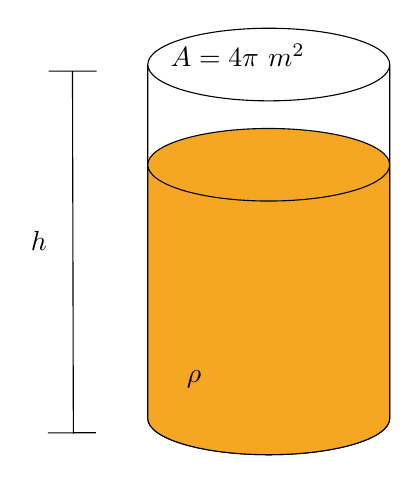
\begin{tikzpicture}[x=0.75pt,y=0.75pt,yscale=-1.2,xscale=1.2]
			%uncomment if require: \path (0,436); %set diagram left start at 0, and has height of 436
			
			%Shape: Can [id:dp6475677626751992] 
			\draw   (197.54,137.57) -- (197.54,279.66) .. controls (197.54,287.71) and (175.79,294.23) .. (148.96,294.23) .. controls (122.13,294.23) and (100.38,287.71) .. (100.38,279.66) -- (100.38,137.57) .. controls (100.38,129.52) and (122.13,123) .. (148.96,123) .. controls (175.79,123) and (197.54,129.52) .. (197.54,137.57) .. controls (197.54,145.62) and (175.79,152.15) .. (148.96,152.15) .. controls (122.13,152.15) and (100.38,145.62) .. (100.38,137.57) ;
			%Straight Lines [id:da23986802958267184] 
			\draw    (60.54,140.23) -- (79.8,140.2) ;
			%Straight Lines [id:da32078657782594644] 
			\draw    (60.23,285.45) -- (79.49,285.42) ;
			%Straight Lines [id:da5428086780456078] 
			\draw    (70.15,140.26) -- (70.5,285.75) ;
			%Shape: Can [id:dp32351772096576803] 
			\draw  [color={rgb, 255:red, 0; green, 0; blue, 0 }  ,draw opacity=1 ][fill={rgb, 255:red, 245; green, 166; blue, 35 }  ,fill opacity=1 ] (197.5,177.82) -- (197.5,279.66) .. controls (197.5,287.71) and (175.76,294.23) .. (148.94,294.23) .. controls (122.12,294.23) and (100.38,287.71) .. (100.38,279.66) -- (100.38,177.82) .. controls (100.38,169.77) and (122.12,163.25) .. (148.94,163.25) .. controls (175.76,163.25) and (197.5,169.77) .. (197.5,177.82) .. controls (197.5,185.86) and (175.76,192.38) .. (148.94,192.38) .. controls (122.12,192.38) and (100.38,185.86) .. (100.38,177.82) ;
			
			% Text Node
			\draw (52.38,203.39) node [anchor=north west][inner sep=0.75pt]    {$h$};
			% Text Node
			\draw (108.5,128.4) node [anchor=north west][inner sep=0.75pt]    {$A=4\pi \ m^{2}$};
			% Text Node
			\draw (115,259.4) node [anchor=north west][inner sep=0.75pt]    {$\rho $};
			
			
		\end{tikzpicture}
	
\caption{Example of a rocket fuel tank}
\label{fig:tanque}
\end{figure}

Consider that both the fluid and the container are ejected at a velocity of $u=4\text{ km/s}$, and that the mass of the circular caps can be neglected, and that the mass of the capsule is $m=10\text{ kg}$ (the only part that will land on the ground). Also consider that even though all the fuel, when activated, is ejected, the spacecraft pilot has full control over the direction of the thrust, and can even adjust the direction during the impulse.

In the case of the ion engine, the ionization chamber stores the atoms and ions at a pressure of 10 atm and a temperature of 73.88 K. It is known that the material constituting the chamber is the same as that of the combustion containers, and the chamber also has the same specifications. The gas constant is $R = 8.314\text{ S.I.}$\footnote{Out of laziness, the author did not explicitly write the units} and the molar mass of Xe is $M = 131.3 \text{ g/mol}$. The containers are ejected at the same velocity as the gas.

\ut{E.4} Determine the total mass, in tons, of the rocket at the moment of launch. Use the velocity equation for non-relativistic cases.

\clearpage

\fi

\ifsolution

\section{Apollo XXVI}

\parte{A}{``Optical'' Rocket}

\ut{A.1} Consider the schematic in Figure \ref{fig:lente}:
        
	\begin{figure}[htpb]
	\centering
	\tikzset{every picture/.style={line width=0.75pt}} %set default line width to 0.75pt
	
		\begin{tikzpicture}[x=0.75pt,y=0.75pt,yscale=-1,xscale=1]
			%uncomment if require: \path (0,436); %set diagram left start at 0, and has height of 436
			
			%Shape: Arc [id:dp5744082319840502] 
			\draw  [draw opacity=0] (170.29,337) .. controls (162.79,322.6) and (157.63,292.26) .. (157.63,257.17) .. controls (157.63,221.76) and (162.89,191.19) .. (170.5,176.95) -- (180.13,257.17) -- cycle ; \draw   (170.29,337) .. controls (162.79,322.6) and (157.63,292.26) .. (157.63,257.17) .. controls (157.63,221.76) and (162.89,191.19) .. (170.5,176.95) ;
			%Shape: Arc [id:dp22587819058871905] 
			\draw  [draw opacity=0] (169.91,176.8) .. controls (178.39,189.12) and (184.41,220.46) .. (184.41,257.18) .. controls (184.41,293.35) and (178.57,324.31) .. (170.29,337) -- (161.91,257.18) -- cycle ; \draw   (169.91,176.8) .. controls (178.39,189.12) and (184.41,220.46) .. (184.41,257.18) .. controls (184.41,293.35) and (178.57,324.31) .. (170.29,337) ;
			%Straight Lines [id:da19948728801956128] 
			\draw  [dash pattern={on 0.84pt off 2.51pt}]  (59.2,261.1) -- (404.64,259.93) ;
			%Straight Lines [id:da9864750725987359] 
			\draw    (109.86,220.21) -- (167.8,220.88) ;
			\draw [shift={(169.8,220.9)}, rotate = 180.66] [color={rgb, 255:red, 0; green, 0; blue, 0 }  ][line width=0.75]    (10.93,-3.29) .. controls (6.95,-1.4) and (3.31,-0.3) .. (0,0) .. controls (3.31,0.3) and (6.95,1.4) .. (10.93,3.29)   ;
			%Straight Lines [id:da8834712071728019] 
			\draw    (169.8,220.9) -- (222.13,233.83) -- (338.16,259.5) ;
			\draw [shift={(340.11,259.93)}, rotate = 192.48] [color={rgb, 255:red, 0; green, 0; blue, 0 }  ][line width=0.75]    (10.93,-3.29) .. controls (6.95,-1.4) and (3.31,-0.3) .. (0,0) .. controls (3.31,0.3) and (6.95,1.4) .. (10.93,3.29)   ;
			%Straight Lines [id:da8279719463080402] 
			\draw    (110,300.21) -- (167.5,300.83) ;
			\draw [shift={(169.5,300.85)}, rotate = 180.61] [color={rgb, 255:red, 0; green, 0; blue, 0 }  ][line width=0.75]    (10.93,-3.29) .. controls (6.95,-1.4) and (3.31,-0.3) .. (0,0) .. controls (3.31,0.3) and (6.95,1.4) .. (10.93,3.29)   ;
			%Straight Lines [id:da5652535893675268] 
			\draw    (169.5,300.85) -- (220.39,287.07) -- (338.16,260.38) ;
			\draw [shift={(340.11,259.93)}, rotate = 167.23] [color={rgb, 255:red, 0; green, 0; blue, 0 }  ][line width=0.75]    (10.93,-3.29) .. controls (6.95,-1.4) and (3.31,-0.3) .. (0,0) .. controls (3.31,0.3) and (6.95,1.4) .. (10.93,3.29)   ;
			%Straight Lines [id:da8153548168326457] 
			\draw    (170.44,170.39) -- (340.22,170.5) ;
			%Straight Lines [id:da27895623213235865] 
			\draw    (170.22,167.28) -- (170.33,173.39) ;
			%Straight Lines [id:da3704898421797518] 
			\draw    (340,167.39) -- (340.11,173.5) ;
			%Straight Lines [id:da3764427895064717] 
			\draw    (387.25,259.81) -- (387.36,180.6) ;
			%Straight Lines [id:da8206980909755612] 
			\draw    (383.58,260) -- (389.69,259.95) ;
			%Straight Lines [id:da5752594624712339] 
			\draw    (384.25,180.7) -- (390.36,180.65) ;
			%Straight Lines [id:da21969419418827463] 
			\draw    (91.29,260.52) -- (91.04,220.42) ;
			%Straight Lines [id:da858659873928072] 
			\draw    (88.18,261.03) -- (94.29,261) ;
			%Straight Lines [id:da6446634861133131] 
			\draw    (87.85,220.24) -- (93.96,220.21) ;
			
			% Text Node
			\draw (247.2,149.2) node [anchor=north west][inner sep=0.75pt]    {$f$};
			% Text Node
			\draw (393.2,210.4) node [anchor=north west][inner sep=0.75pt]    {$R$};
			% Text Node
			\draw (78,232.8) node [anchor=north west][inner sep=0.75pt]    {$x$};
			
			
		\end{tikzpicture}
	
\caption{Lens and convergence of light rays}
\label{fig:lente}
\end{figure}

Considering the radiation passing through the lens within the range of rays $x$ to $x+dx$, the power transmitted under these conditions is: $L=F_\odot 2\pi x dx$. The energy is then described over an exposure time $dt$: $E=2\pi F_\odot x dx dt$. Using Einstein's relation for photons, we know that $E=pc$, where $p$ is the momentum of the radiation. Thus, we can find the initial momentum of the photons passing through the lens under these conditions: $p=\frac{2\pi F_\odot}{c}xdxdt$.

After passing through the lens, this same momentum is redirected toward the focus, so that the momentum in the original direction of motion is $p\cos{(\theta)}$, where $\theta$ is the deflection angle, such that $\tan{(\theta)}=\dfrac{x}{f}$, with $f$ being the focal length. Therefore, the change in momentum along the horizontal axis\footnote{The change in momentum along axes perpendicular to the horizontal is zero, due to the cylindrical symmetry of the lens} is $dp=p(\cos{(\theta)}-1)$. By conservation of momentum, the change in momentum of the lens is $dp=p(1-\cos{(\theta)})$:

$$\cos{(\theta)}=\frac{1}{\sqrt{1+\tan^2{(\theta)}}}$$

$$dp=\frac{2\pi F_\odot}{c}xdxdt\left( 1-\frac{f}{\sqrt{f^2+x^2}}\right) $$

Integrating over all values of $x$:

$$\int_0^dp_xdp=\frac{2\pi F_\odot}{c}dt\int_0^R\left( 1-\frac{f}{\sqrt{f^2+x^2}}\right) xdx$$

$$\frac{cdp_x}{2\pi F_\odot dt}=\int_0^Rxdx-\int_0^R\frac{xdx}{\sqrt{1+\frac{x^2}{f^2}}}$$

Substituting $u=1+x^2/f^2$ ($du=2xdx/f^2$):

$$\frac{cdp_x}{2\pi F_\odot dt}=\frac{R^2}{2}-\frac{f^2}{2}\int_1^{1+\frac{R^2}{f^2}}\frac{du}{\sqrt{u}}$$

Solving, we find:

$$\frac{cdp_x}{2\pi F_\odot dt}=\frac{R^2}{2}-f^2\left(\sqrt{1+\frac{R^2}{f^2}}-1 \right) $$

Using the known focal ratio, we have $\frac{f}{D}=\frac{f}{2R}=\beta$. Substituting this into the previous result and simplifying slightly:

$$dp_x=\frac{2\pi F_\odot R^2}{c}\left(\frac{1}{2}-2\beta\left( \sqrt{4\beta^2+1}-2\beta\right)  \right)dt $$

By the definition of force, $F_x=\dfrac{dp_x}{dt}$, so:

$$F_x=\frac{2\pi F_\odot R^2}{c}\left(\frac{1}{2}-2\beta\left( \sqrt{4\beta^2+1}-2\beta\right)  \right)$$

\ut{A.2} Substituting the values, we find the desired answer: $\Delta t \approx 357.4\text{ years}$.

\ut{A.3} Note that the force $F_x$ can be written as $F_x=kF_\odot=k\frac{L_\odot}{4\pi r^2}$, where $r$ is the distance from the satellite to the center of the star. To balance the gravitational force, we want:

$$\frac{ L_\odot R^2}{2r^2c}\left(\frac{1}{2}-2\beta\left( \sqrt{4\beta^2+1}-2\beta\right)  \right)=\frac{GMm}{r^2}$$

$$M=\frac{ L_\odot R^2}{2Gmc}\left(\frac{1}{2}-2\beta\left( \sqrt{4\beta^2+1}-2\beta\right)  \right)$$

In this case, $M=6.72\cdot10^{19}\text{ kg}$, approximately a thousand times lighter than the Moon!

\parte{B}{Mass Cannon}

\ut{B.1} To solve this problem, it is useful to first move to the reference frame of the moving body, where the parameters are easier to understand, and then apply the necessary transformations. In this problem, we will denote the reference frame $S$ as that of the moving spacecraft\footnote{Note the interesting fact that the reference frame $S$ is accelerated, since it follows the spacecraft; however, we will consider a $dt$ over which the spacecraft's velocity is practically constant and work in this regime.}, while $S'$ is for an inertial observer outside the spacecraft.

For this, consider the following scheme in reference frame $S$.


	\begin{figure}[htpb]
	\centering
		
		\tikzset{every picture/.style={line width=0.75pt}} %set default line width to 0.75pt        
		
		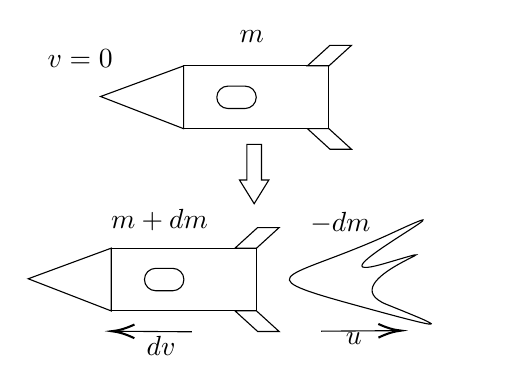
\begin{tikzpicture}[x=0.75pt,y=0.75pt,yscale=-1,xscale=1]
			%uncomment if require: \path (0,436); %set diagram left start at 0, and has height of 436
			
			%Shape: Triangle [id:dp6812826884823431] 
			\draw   (60.5,224.88) -- (100.5,210.13) -- (100.5,240.38) -- cycle ;
			%Rounded Rect [id:dp04995433603772059] 
			\draw   (100.5,210.13) .. controls (100.5,210.13) and (100.5,210.13) .. (100.5,210.13) -- (170.5,210.13) .. controls (170.5,210.13) and (170.5,210.13) .. (170.5,210.13) -- (170.5,240.38) .. controls (170.5,240.38) and (170.5,240.38) .. (170.5,240.38) -- (100.5,240.38) .. controls (100.5,240.38) and (100.5,240.38) .. (100.5,240.38) -- cycle ;
			%Shape: Rectangle [id:dp37291835601379764] 
			\draw   (171,200.22) -- (181.39,200.22) -- (170.5,210.13) -- (160.11,210.13) -- cycle ;
			%Shape: Rectangle [id:dp6692566306060299] 
			\draw   (170.5,240.38) -- (160.16,240.38) -- (171.06,250.29) -- (181.4,250.29) -- cycle ;
			%Rounded Rect [id:dp7395147077133022] 
			\draw   (116.5,225.25) .. controls (116.5,222.27) and (118.92,219.85) .. (121.9,219.85) -- (130.1,219.85) .. controls (133.08,219.85) and (135.5,222.27) .. (135.5,225.25) -- (135.5,225.25) .. controls (135.5,228.23) and (133.08,230.65) .. (130.1,230.65) -- (121.9,230.65) .. controls (118.92,230.65) and (116.5,228.23) .. (116.5,225.25) -- cycle ;
			%Shape: Polygon Curved [id:ds3584543864907703] 
			\draw   (236.71,202.43) .. controls (285.29,179.86) and (189.29,230.14) .. (233,217.29) .. controls (276.71,204.43) and (204.14,225.57) .. (233.29,237.29) .. controls (262.43,249) and (266.71,251) .. (215,236.71) .. controls (163.29,222.43) and (188.14,225) .. (236.71,202.43) -- cycle ;
			%Shape: Triangle [id:dp9932731179533096] 
			\draw   (95.36,137.07) -- (135.36,122.32) -- (135.36,152.57) -- cycle ;
			%Rounded Rect [id:dp6609156462545449] 
			\draw   (135.36,122.32) .. controls (135.36,122.32) and (135.36,122.32) .. (135.36,122.32) -- (205.36,122.32) .. controls (205.36,122.32) and (205.36,122.32) .. (205.36,122.32) -- (205.36,152.57) .. controls (205.36,152.57) and (205.36,152.57) .. (205.36,152.57) -- (135.36,152.57) .. controls (135.36,152.57) and (135.36,152.57) .. (135.36,152.57) -- cycle ;
			%Shape: Rectangle [id:dp92879960110657] 
			\draw   (205.86,112.41) -- (216.25,112.41) -- (205.36,122.32) -- (194.97,122.32) -- cycle ;
			%Shape: Rectangle [id:dp20436309141585207] 
			\draw   (205.36,152.57) -- (195.02,152.57) -- (205.92,162.49) -- (216.26,162.49) -- cycle ;
			%Rounded Rect [id:dp9110273349462445] 
			\draw   (151.36,137.45) .. controls (151.36,134.46) and (153.77,132.05) .. (156.76,132.05) -- (164.96,132.05) .. controls (167.94,132.05) and (170.36,134.46) .. (170.36,137.45) -- (170.36,137.45) .. controls (170.36,140.43) and (167.94,142.85) .. (164.96,142.85) -- (156.76,142.85) .. controls (153.77,142.85) and (151.36,140.43) .. (151.36,137.45) -- cycle ;
			%Down Arrow [id:dp9122136897496416] 
			\draw   (162.29,177.29) -- (165.82,177.29) -- (165.82,160.14) -- (172.89,160.14) -- (172.89,177.29) -- (176.43,177.29) -- (169.36,188.71) -- cycle ;
			%Straight Lines [id:da8761299773449813] 
			\draw    (139.29,250.43) -- (102.71,250.16) ;
			\draw [shift={(100.71,250.14)}, rotate = 0.42] [color={rgb, 255:red, 0; green, 0; blue, 0 }  ][line width=0.75]    (10.93,-3.29) .. controls (6.95,-1.4) and (3.31,-0.3) .. (0,0) .. controls (3.31,0.3) and (6.95,1.4) .. (10.93,3.29)   ;
			%Straight Lines [id:da7368040131336955] 
			\draw    (201.57,250.14) -- (238.14,249.87) ;
			\draw [shift={(240.14,249.86)}, rotate = 179.58] [color={rgb, 255:red, 0; green, 0; blue, 0 }  ][line width=0.75]    (10.93,-3.29) .. controls (6.95,-1.4) and (3.31,-0.3) .. (0,0) .. controls (3.31,0.3) and (6.95,1.4) .. (10.93,3.29)   ;
			
			% Text Node
			\draw (161.14,104.17) node [anchor=north west][inner sep=0.75pt]    {$m$};
			% Text Node
			\draw (68.57,113.32) node [anchor=north west][inner sep=0.75pt]    {$v=0$};
			% Text Node
			\draw (99.14,190.03) node [anchor=north west][inner sep=0.75pt]    {$m+dm$};
			% Text Node
			\draw (195.14,191.46) node [anchor=north west][inner sep=0.75pt]    {$-dm$};
			% Text Node
			\draw (116.29,251.46) node [anchor=north west][inner sep=0.75pt]    {$dv$};
			% Text Node
			\draw (212.29,249.74) node [anchor=north west][inner sep=0.75pt]    {$u$};
			
			
		\end{tikzpicture}
		
\caption{Operating principle of a mass-ejection rocket}
\end{figure}

The spacecraft has a mass $m$ at a generic instant $t$, and at a time $dt$ later, its mass is $dm$. Note that $dm<0$, so we must consider that the mass released is actually $-dm$. By conservation of linear momentum (initially $p=0$):

$$0=(m+dm)(dv)\frac{1}{\sqrt{1-\frac{u^2}{c^2}}}-(-dm)u\frac{1}{\sqrt{1-\frac{u^2}{c^2}}}$$

Ignoring terms containing the product of two infinitesimals and approximating the Lorentz factor for $dv$ as $1$, we have:

$$mdv=-\frac{udm}{\sqrt{1-\frac{u^2}{c^2}}}$$

$$dv=-\frac{udm}{m\sqrt{1-\frac{u^2}{c^2}}}$$

Having done this analysis, we must transfer this result to reference frame $S'$ in order to find $dv'$, i.e., the differential velocity in $S'$.

By the Lorentz transformations, from the velocity $v$ of a point moving along the $x$-axis in both frames, we can find the velocity $v'$ of the same point in $S'$, with $V$ being the velocity of the spacecraft relative to $S'$:

$$
\begin{cases}
	dx'=\gamma(x+Vt)\\
	dt'=\gamma\left(t+\frac{Vx}{c^2}\right)\\
\end{cases}
$$

Dividing both equations:

$$v'=\frac{dx+Vdt}{dt+\frac{Vdx}{c^2}}=\frac{v+V}{1+\frac{Vv}{c^2}}$$

Differentiating both sides allows us to relate the changes in velocities:

$$dv'=\frac{\left(1+\frac{Vv}{c^2} \right) dv-(v+V)\frac{V}{c^2}dv}{\left(1+\frac{Vv}{c^2} \right)^2 }$$

Now consider that this "random" point is the spacecraft after the addition of $dv$, our object of interest. In this case: $v'=V$ and $v=0$:

$$dV=dv-\frac{V^2}{c^2}dv=\left(1-\frac{V^2}{c^2} \right)dv $$

$$\frac{dV}{1-\frac{V^2}{c^2} }=-\frac{udm}{m\sqrt{1-\frac{u^2}{c^2}}}$$

$$\int_0^{V(t)}\frac{dV}{1-\frac{V^2}{c^2} }=-\int_{m_0}^{m(t)}\frac{udm}{m\sqrt{1-\frac{u^2}{c^2}}}$$

Substitute $y=V/c$:

$$c\int_0^{\frac{V}{c}}\frac{dy}{1-y^2 }=-\frac{u}{\sqrt{1-\frac{u^2}{c^2}}}\int_{m_0}^{m(t)}\frac{dm}{m}$$

The following integrals are well known and result in $\tanh^{-1}{(y)}$ and $\ln{(m)}$, respectively:

$$\tanh^{-1}{\left( \frac{V(t)}{c}\right) }=-\frac{u}{c\sqrt{1-\frac{u^2}{c^2}}}\ln{\left(\frac{m(t)}{m_0} \right) }$$

Finally:

$$V(t)=\tanh{\left(-\frac{u}{\sqrt{c^2-u^2}}\ln{(f(t))} \right) }c$$

\ut{B.2} In the classical limit $c\rightarrow \infty$, the argument of the hyperbolic tangent tends to $0$. The function $\tanh{(x)}$ can be written as:

$$\tanh{(x)}=\frac{e^x-e^{-x}}{e^x+e^{-x}}$$

Taking $x\rightarrow0$: $e^x\rightarrow1+x$ (Taylor expansion), so:

$$\tanh{(x)}\rightarrow\frac{1+x-1+x}{1+x+1-x}=x$$

Therefore:

$$V(t)=-\frac{uc}{\sqrt{c^2-u^2}}\ln{(f(t))}$$

Since $u\ll c$:

$$V(t)=-u\ln{(f(t))}$$

\parte{C}{Radiation Cannon}

We will use the same technique described in part B. Consider the spacecraft emitting radiation as follows:

	\begin{figure}[htpb]
		\centering
		
		\tikzset{every picture/.style={line width=0.75pt}} %set default line width to 0.75pt        
		
		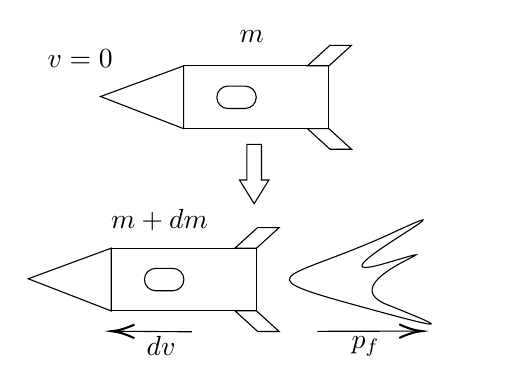
\begin{tikzpicture}[x=0.75pt,y=0.75pt,yscale=-1,xscale=1]
			%uncomment if require: \path (0,436); %set diagram left start at 0, and has height of 436
			
			%Shape: Triangle [id:dp6812826884823431] 
			\draw   (60.5,224.88) -- (100.5,210.13) -- (100.5,240.38) -- cycle ;
			%Rounded Rect [id:dp04995433603772059] 
			\draw   (100.5,210.13) .. controls (100.5,210.13) and (100.5,210.13) .. (100.5,210.13) -- (170.5,210.13) .. controls (170.5,210.13) and (170.5,210.13) .. (170.5,210.13) -- (170.5,240.38) .. controls (170.5,240.38) and (170.5,240.38) .. (170.5,240.38) -- (100.5,240.38) .. controls (100.5,240.38) and (100.5,240.38) .. (100.5,240.38) -- cycle ;
			%Shape: Rectangle [id:dp37291835601379764] 
			\draw   (171,200.22) -- (181.39,200.22) -- (170.5,210.13) -- (160.11,210.13) -- cycle ;
			%Shape: Rectangle [id:dp6692566306060299] 
			\draw   (170.5,240.38) -- (160.16,240.38) -- (171.06,250.29) -- (181.4,250.29) -- cycle ;
			%Rounded Rect [id:dp7395147077133022] 
			\draw   (116.5,225.25) .. controls (116.5,222.27) and (118.92,219.85) .. (121.9,219.85) -- (130.1,219.85) .. controls (133.08,219.85) and (135.5,222.27) .. (135.5,225.25) -- (135.5,225.25) .. controls (135.5,228.23) and (133.08,230.65) .. (130.1,230.65) -- (121.9,230.65) .. controls (118.92,230.65) and (116.5,228.23) .. (116.5,225.25) -- cycle ;
			%Shape: Polygon Curved [id:ds3584543864907703] 
			\draw   (236.71,202.43) .. controls (285.29,179.86) and (189.29,230.14) .. (233,217.29) .. controls (276.71,204.43) and (204.14,225.57) .. (233.29,237.29) .. controls (262.43,249) and (266.71,251) .. (215,236.71) .. controls (163.29,222.43) and (188.14,225) .. (236.71,202.43) -- cycle ;
			%Shape: Triangle [id:dp9932731179533096] 
			\draw   (95.36,137.07) -- (135.36,122.32) -- (135.36,152.57) -- cycle ;
			%Rounded Rect [id:dp6609156462545449] 
			\draw   (135.36,122.32) .. controls (135.36,122.32) and (135.36,122.32) .. (135.36,122.32) -- (205.36,122.32) .. controls (205.36,122.32) and (205.36,122.32) .. (205.36,122.32) -- (205.36,152.57) .. controls (205.36,152.57) and (205.36,152.57) .. (205.36,152.57) -- (135.36,152.57) .. controls (135.36,152.57) and (135.36,152.57) .. (135.36,152.57) -- cycle ;
			%Shape: Rectangle [id:dp92879960110657] 
			\draw   (205.86,112.41) -- (216.25,112.41) -- (205.36,122.32) -- (194.97,122.32) -- cycle ;
			%Shape: Rectangle [id:dp20436309141585207] 
			\draw   (205.36,152.57) -- (195.02,152.57) -- (205.92,162.49) -- (216.26,162.49) -- cycle ;
			%Rounded Rect [id:dp9110273349462445] 
			\draw   (151.36,137.45) .. controls (151.36,134.46) and (153.77,132.05) .. (156.76,132.05) -- (164.96,132.05) .. controls (167.94,132.05) and (170.36,134.46) .. (170.36,137.45) -- (170.36,137.45) .. controls (170.36,140.43) and (167.94,142.85) .. (164.96,142.85) -- (156.76,142.85) .. controls (153.77,142.85) and (151.36,140.43) .. (151.36,137.45) -- cycle ;
			%Down Arrow [id:dp9122136897496416] 
			\draw   (162.29,177.29) -- (165.82,177.29) -- (165.82,160.14) -- (172.89,160.14) -- (172.89,177.29) -- (176.43,177.29) -- (169.36,188.71) -- cycle ;
			%Straight Lines [id:da8761299773449813] 
			\draw    (139.29,250.43) -- (102.71,250.16) ;
			\draw [shift={(100.71,250.14)}, rotate = 0.42] [color={rgb, 255:red, 0; green, 0; blue, 0 }  ][line width=0.75]    (10.93,-3.29) .. controls (6.95,-1.4) and (3.31,-0.3) .. (0,0) .. controls (3.31,0.3) and (6.95,1.4) .. (10.93,3.29)   ;
			%Straight Lines [id:da4662318384394215] 
			\draw    (199.8,250.2) -- (248.2,250.1) ;
			\draw [shift={(250.2,250.1)}, rotate = 179.89] [color={rgb, 255:red, 0; green, 0; blue, 0 }  ][line width=0.75]    (10.93,-3.29) .. controls (6.95,-1.4) and (3.31,-0.3) .. (0,0) .. controls (3.31,0.3) and (6.95,1.4) .. (10.93,3.29)   ;
			
			% Text Node
			\draw (161.14,104.17) node [anchor=north west][inner sep=0.75pt]    {$m$};
			% Text Node
			\draw (68.57,113.32) node [anchor=north west][inner sep=0.75pt]    {$v=0$};
			% Text Node
			\draw (99.14,190.03) node [anchor=north west][inner sep=0.75pt]    {$m+dm$};
			% Text Node
			\draw (116.29,251.46) node [anchor=north west][inner sep=0.75pt]    {$dv$};
			% Text Node
			\draw (215,251.46) node [anchor=north west][inner sep=0.75pt]    {$p_f$};
			
			
		\end{tikzpicture}
	
\caption{Operating principle of a photon-ejection rocket}
\end{figure}

From the conservation of linear momentum we can conclude:

$$0=(m+dm)dv-p_f$$

However, using Einstein's energy-momentum relation for photons, we have $E=pc$:

$$(m+dm)dv=\frac{E}{c}$$

Now, by conservation of the total energy of the system\footnote{Since the rocket's speed increased only infinitesimally, its total energy is basically contained in the rest energy}:

$$mc^2=(m+dm)c^2+E \rightarrow E=-c^2dm$$

$$\therefore mdv = dmc \rightarrow dv = -\frac{dm}{m}c$$

Using the reference frame transformation demonstrated in item B:

$$dV = \left(1-\frac{V^2}{c^2} \right) dv$$

$$\frac{dV}{1-\frac{V^2}{c^2}} = -\frac{dm}{m}c$$

Integrating the previous equation:

$$c \tanh^{-1}{\left( \frac{V(t)}{c}\right) } = -c \ln{\left(f(t)\right) }$$

$$\therefore V(t) = \tanh{(\ln{(f(t))})} c$$

However, as shown previously:

$$\tanh{(-\ln(f(t)))} = \frac{e^{-\ln{(f(t))}} - e^{\ln{(f(t))}}}{e^{-\ln{(f(t))}} + e^{\ln{(f(t))}}} = \frac{-f(t) + \frac{1}{f(t)}}{f(t) + \frac{1}{f(t)}}$$

Simplifying the expression we find:

$$V(t) = \frac{1 - (f(t))^2}{1 + (f(t))^2} c$$

\parte{D}{Ion Propulsion}

\ut{D.1} The walls of the ionization chamber are electrified both to attract the remaining electrons from the reaction and to "guide" the Xe$^+$ cations towards the acceleration plates, as well as to prevent collisions with the walls which, due to their high velocity, could damage the chamber structure.

\ut{D.2} To calculate the electric field between the plates, we use Gauss's law:

$$\oint_S \vec{E} \cdot \vec{dA} = \frac{q}{\epsilon_0}$$

Consider the following setup with a cylindrical analysis surface:

	\begin{figure}[htpb]
	\centering
		
		\tikzset{every picture/.style={line width=0.75pt}} %set default line width to 0.75pt        
		
		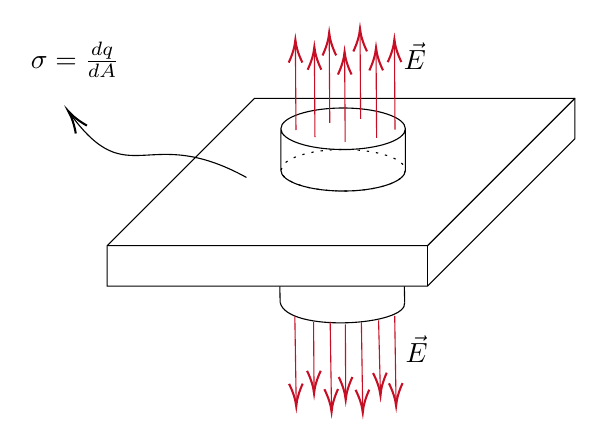
\begin{tikzpicture}[x=0.75pt,y=0.75pt,yscale=-1,xscale=1]
			%uncomment if require: \path (0,436); %set diagram left start at 0, and has height of 436
			
			%Shape: Can [id:dp16042671032465616] 
			\draw   (350,181.83) -- (350,201.83) .. controls (350,207.36) and (336.57,211.83) .. (320,211.83) .. controls (303.43,211.83) and (290,207.36) .. (290,201.83) -- (290,181.83) .. controls (290,176.31) and (303.43,171.83) .. (320,171.83) .. controls (336.57,171.83) and (350,176.31) .. (350,181.83) .. controls (350,187.36) and (336.57,191.83) .. (320,191.83) .. controls (303.43,191.83) and (290,187.36) .. (290,181.83) ;
			%Shape: Cube [id:dp44459967660773203] 
			\draw   (206.33,238.17) -- (277.33,167.17) -- (431.67,167.17) -- (431.67,186.67) -- (360.67,257.67) -- (206.33,257.67) -- cycle ; \draw   (431.67,167.17) -- (360.67,238.17) -- (206.33,238.17) ; \draw   (360.67,238.17) -- (360.67,257.67) ;
			%Straight Lines [id:da6216463203261222] 
			\draw    (289.5,257.75) -- (289.66,265.5) ;
			%Straight Lines [id:da32697913773783127] 
			\draw    (349.5,257.75) -- (349.66,265.5) ;
			%Curve Lines [id:da6223919224562344] 
			\draw    (289.66,265.5) .. controls (292.83,280.25) and (351.33,276.92) .. (349.66,265.5) ;
			%Shape: Ellipse [id:dp29648724822139094] 
			\draw  [dash pattern={on 0.84pt off 2.51pt}] (290.14,201.83) .. controls (290.14,196.31) and (303.54,191.83) .. (320.07,191.83) .. controls (336.6,191.83) and (350,196.31) .. (350,201.83) .. controls (350,207.36) and (336.6,211.83) .. (320.07,211.83) .. controls (303.54,211.83) and (290.14,207.36) .. (290.14,201.83) -- cycle ;
			%Curve Lines [id:da3151246823467999] 
			\draw    (273.43,205.29) .. controls (225.2,178.7) and (216.88,213.71) .. (188.44,174.5) ;
			\draw [shift={(187.57,173.29)}, rotate = 54.69] [color={rgb, 255:red, 0; green, 0; blue, 0 }  ][line width=0.75]    (10.93,-3.29) .. controls (6.95,-1.4) and (3.31,-0.3) .. (0,0) .. controls (3.31,0.3) and (6.95,1.4) .. (10.93,3.29)   ;
			%Straight Lines [id:da7002484547488983] 
			\draw [color={rgb, 255:red, 198; green, 15; blue, 37 }  ,draw opacity=1 ]   (297.29,182.43) -- (297.01,141) ;
			\draw [shift={(297,139)}, rotate = 89.62] [color={rgb, 255:red, 198; green, 15; blue, 37 }  ,draw opacity=1 ][line width=0.75]    (10.93,-3.29) .. controls (6.95,-1.4) and (3.31,-0.3) .. (0,0) .. controls (3.31,0.3) and (6.95,1.4) .. (10.93,3.29)   ;
			%Straight Lines [id:da29004940971374604] 
			\draw [color={rgb, 255:red, 198; green, 15; blue, 37 }  ,draw opacity=1 ]   (321,188.2) -- (320.73,146.77) ;
			\draw [shift={(320.71,144.77)}, rotate = 89.62] [color={rgb, 255:red, 198; green, 15; blue, 37 }  ,draw opacity=1 ][line width=0.75]    (10.93,-3.29) .. controls (6.95,-1.4) and (3.31,-0.3) .. (0,0) .. controls (3.31,0.3) and (6.95,1.4) .. (10.93,3.29)   ;
			%Straight Lines [id:da6203069568332062] 
			\draw [color={rgb, 255:red, 198; green, 15; blue, 37 }  ,draw opacity=1 ]   (328.43,177.06) -- (328.16,135.63) ;
			\draw [shift={(328.14,133.63)}, rotate = 89.62] [color={rgb, 255:red, 198; green, 15; blue, 37 }  ,draw opacity=1 ][line width=0.75]    (10.93,-3.29) .. controls (6.95,-1.4) and (3.31,-0.3) .. (0,0) .. controls (3.31,0.3) and (6.95,1.4) .. (10.93,3.29)   ;
			%Straight Lines [id:da20918800286291983] 
			\draw [color={rgb, 255:red, 198; green, 15; blue, 37 }  ,draw opacity=1 ]   (336.14,186.2) -- (335.87,144.77) ;
			\draw [shift={(335.86,142.77)}, rotate = 89.62] [color={rgb, 255:red, 198; green, 15; blue, 37 }  ,draw opacity=1 ][line width=0.75]    (10.93,-3.29) .. controls (6.95,-1.4) and (3.31,-0.3) .. (0,0) .. controls (3.31,0.3) and (6.95,1.4) .. (10.93,3.29)   ;
			%Straight Lines [id:da2701830161797232] 
			\draw [color={rgb, 255:red, 198; green, 15; blue, 37 }  ,draw opacity=1 ]   (345,182.2) -- (344.73,140.77) ;
			\draw [shift={(344.71,138.77)}, rotate = 89.62] [color={rgb, 255:red, 198; green, 15; blue, 37 }  ,draw opacity=1 ][line width=0.75]    (10.93,-3.29) .. controls (6.95,-1.4) and (3.31,-0.3) .. (0,0) .. controls (3.31,0.3) and (6.95,1.4) .. (10.93,3.29)   ;
			%Straight Lines [id:da24324087641122327] 
			\draw [color={rgb, 255:red, 198; green, 15; blue, 37 }  ,draw opacity=1 ]   (313.57,179) -- (313.3,137.57) ;
			\draw [shift={(313.29,135.57)}, rotate = 89.62] [color={rgb, 255:red, 198; green, 15; blue, 37 }  ,draw opacity=1 ][line width=0.75]    (10.93,-3.29) .. controls (6.95,-1.4) and (3.31,-0.3) .. (0,0) .. controls (3.31,0.3) and (6.95,1.4) .. (10.93,3.29)   ;
			%Straight Lines [id:da32040811248710144] 
			\draw [color={rgb, 255:red, 198; green, 15; blue, 37 }  ,draw opacity=1 ]   (306.43,185.86) -- (306.16,144.43) ;
			\draw [shift={(306.14,142.43)}, rotate = 89.62] [color={rgb, 255:red, 198; green, 15; blue, 37 }  ,draw opacity=1 ][line width=0.75]    (10.93,-3.29) .. controls (6.95,-1.4) and (3.31,-0.3) .. (0,0) .. controls (3.31,0.3) and (6.95,1.4) .. (10.93,3.29)   ;
			%Straight Lines [id:da1845033553659554] 
			\draw [color={rgb, 255:red, 198; green, 15; blue, 37 }  ,draw opacity=1 ]   (344.85,271.93) -- (345.5,313.35) ;
			\draw [shift={(345.53,315.35)}, rotate = 269.1] [color={rgb, 255:red, 198; green, 15; blue, 37 }  ,draw opacity=1 ][line width=0.75]    (10.93,-3.29) .. controls (6.95,-1.4) and (3.31,-0.3) .. (0,0) .. controls (3.31,0.3) and (6.95,1.4) .. (10.93,3.29)   ;
			%Straight Lines [id:da43428951136036353] 
			\draw [color={rgb, 255:red, 198; green, 15; blue, 37 }  ,draw opacity=1 ]   (321.08,276.02) -- (321.24,310.38) ;
			\draw [shift={(321.25,312.38)}, rotate = 269.74] [color={rgb, 255:red, 198; green, 15; blue, 37 }  ,draw opacity=1 ][line width=0.75]    (10.93,-3.29) .. controls (6.95,-1.4) and (3.31,-0.3) .. (0,0) .. controls (3.31,0.3) and (6.95,1.4) .. (10.93,3.29)   ;
			%Straight Lines [id:da9811049379633601] 
			\draw [color={rgb, 255:red, 198; green, 15; blue, 37 }  ,draw opacity=1 ]   (313.76,274.78) -- (314.41,316.21) ;
			\draw [shift={(314.44,318.21)}, rotate = 269.1] [color={rgb, 255:red, 198; green, 15; blue, 37 }  ,draw opacity=1 ][line width=0.75]    (10.93,-3.29) .. controls (6.95,-1.4) and (3.31,-0.3) .. (0,0) .. controls (3.31,0.3) and (6.95,1.4) .. (10.93,3.29)   ;
			%Straight Lines [id:da747747322268409] 
			\draw [color={rgb, 255:red, 198; green, 15; blue, 37 }  ,draw opacity=1 ]   (305.76,274.91) -- (305.99,307.38) ;
			\draw [shift={(306,309.38)}, rotate = 269.6] [color={rgb, 255:red, 198; green, 15; blue, 37 }  ,draw opacity=1 ][line width=0.75]    (10.93,-3.29) .. controls (6.95,-1.4) and (3.31,-0.3) .. (0,0) .. controls (3.31,0.3) and (6.95,1.4) .. (10.93,3.29)   ;
			%Straight Lines [id:da9155982351538259] 
			\draw [color={rgb, 255:red, 198; green, 15; blue, 37 }  ,draw opacity=1 ]   (296.74,272.19) -- (297.39,313.61) ;
			\draw [shift={(297.42,315.61)}, rotate = 269.1] [color={rgb, 255:red, 198; green, 15; blue, 37 }  ,draw opacity=1 ][line width=0.75]    (10.93,-3.29) .. controls (6.95,-1.4) and (3.31,-0.3) .. (0,0) .. controls (3.31,0.3) and (6.95,1.4) .. (10.93,3.29)   ;
			%Straight Lines [id:da4716425680408849] 
			\draw [color={rgb, 255:red, 198; green, 15; blue, 37 }  ,draw opacity=1 ]   (328.8,275.1) -- (329.44,316.53) ;
			\draw [shift={(329.48,318.53)}, rotate = 269.1] [color={rgb, 255:red, 198; green, 15; blue, 37 }  ,draw opacity=1 ][line width=0.75]    (10.93,-3.29) .. controls (6.95,-1.4) and (3.31,-0.3) .. (0,0) .. controls (3.31,0.3) and (6.95,1.4) .. (10.93,3.29)   ;
			%Straight Lines [id:da46483278770216097] 
			\draw [color={rgb, 255:red, 198; green, 15; blue, 37 }  ,draw opacity=1 ]   (337.08,274.18) -- (337.95,308.38) ;
			\draw [shift={(338,310.38)}, rotate = 268.54] [color={rgb, 255:red, 198; green, 15; blue, 37 }  ,draw opacity=1 ][line width=0.75]    (10.93,-3.29) .. controls (6.95,-1.4) and (3.31,-0.3) .. (0,0) .. controls (3.31,0.3) and (6.95,1.4) .. (10.93,3.29)   ;
			
			% Text Node
			\draw (348,139.03) node [anchor=north west][inner sep=0.75pt]    {$\vec{E}$};
			% Text Node
			\draw (348.86,280.37) node [anchor=north west][inner sep=0.75pt]    {$\vec{E}$};
			% Text Node
			\draw (168.29,138.97) node [anchor=north west][inner sep=0.75pt]    {$\sigma =\frac{dq}{dA}$};
			
			
		\end{tikzpicture}
	
\caption{Electric field lines for an "infinite" flat surface. For real objects, an infinite dimension is impossible, however, such a phenomenon can be approximated with a plate much larger than the size of the chosen cylinder, so as to cancel edge effects.}
\end{figure}

Such a cylinder is designed so that its length above and below the plate is equal and it has a cross-sectional area equal to $dA$. The charge inside the surface is simply $dq = \sigma dA$. By symmetry, $\vec{E}$ is constant over the surface, so that:

$$\oint_S \vec{E} \cdot \vec{dA} = \vec{E} \cdot (2 dA) = \frac{\sigma dA}{\epsilon_0}$$

$$\therefore \vec{E} = \frac{\sigma}{2 \epsilon_0} \hat{r}$$

Where $\hat{r}$ is the unit vector pointing in the direction and sense from the point relative to the plate (so that $\vec{E}$ always "leaves" or "enters" the plate, depending on whether the plate has positive or negative charge, respectively).

Thus, between the plates we have:

$$|\vec{E}| = \frac{\sigma_+ - \sigma_-}{2 \epsilon_0}$$

Where $\sigma_+$ and $\sigma_-$ are the surface charge densities of the positive and negative plates, respectively. Note that $\vec{E}$ "points" outward from the engine, perpendicular to the plates!

By the definition of potential:

$$\Delta V = -\int_{r_1}^{r_2} \vec{E} \cdot \vec{dr}$$

$$\therefore |\Delta V| = \frac{\sigma_+ - \sigma_-}{2 \epsilon_0} E$$

\textbf{Note:} Do not confuse the $E$ in the previous equation with the electric field; in this case, it is the distance between the plates!

\ut{D.3} The amount of energy given to the ions passing through the acceleration plates is $\Delta U = q \Delta V$, where $q$ is the charge of an ion ($q = 1 e^- = 1.602\cdot 10^{-19} C$):

$$\frac{mv^2}{2} = q \Delta V$$

$$\therefore v = \sqrt{2\frac{q}{m} \Delta V}$$

$$v = 85.4 \text{ km/s}$$

\ut{D.4} Starting from the relation obtained in part B:

$$\Delta v(t) = -\sqrt{2\frac{q}{m} \Delta V} \ln{(f(t))}$$

\parte{E}{Space Exploration}

\ut{E.1} Each stage will represent a $\Delta v$ for orbital change. A $\Delta v_1$ is needed to enter the transfer orbit to Genibals, performed by the combustion engine (high thrust for vehicle ejection), and a $\Delta v_2$ to exit the transfer orbit and enter the same orbit as Genibals, which will be performed by the ion engine.

A $\Delta v_3$ is needed to land on Genibals, performed by the combustion engine (to counter the high descent speeds), a $\Delta v_4$ to leave Genibals again, also performed by the combustion engine, and a $\Delta v_5$ to enter the transfer orbit, which can be performed by the ion engine.

For the return to Plutão II, a $\Delta v_6$ is needed to enter the same orbit as Plutão II and exit the transfer orbit, performed by the ion engine, and finally a last $\Delta v_7$ to land on Plutão II, performed by the combustion engine.

Thus, the rocket requires \textbf{7 propulsion stages}\footnote{A common question is why the arrival at Genibals and Plutão II, as well as departure from Genibals, is divided into two distinct impulses: one to enter/exit orbit and another to land/enter the transfer orbit. This is because these impulses occur in different directions, so if they were applied at once (as if summed), the spacecraft would have too high a velocity and would enter a different elliptical orbit.}.

\ut{E.2} Notice that, since the rocket is not launched directly from the equator, it will have a certain elevation relative to the orbital plane. Therefore, upon reaching Genibals, this elevation must be taken into account. Analyze the figure beside, which (not to scale) represents the situation:

	\begin{figure}[htpb]
		\centering
		\tikzset{every picture/.style={line width=0.75pt}} %set default line width to 0.75pt        
		
		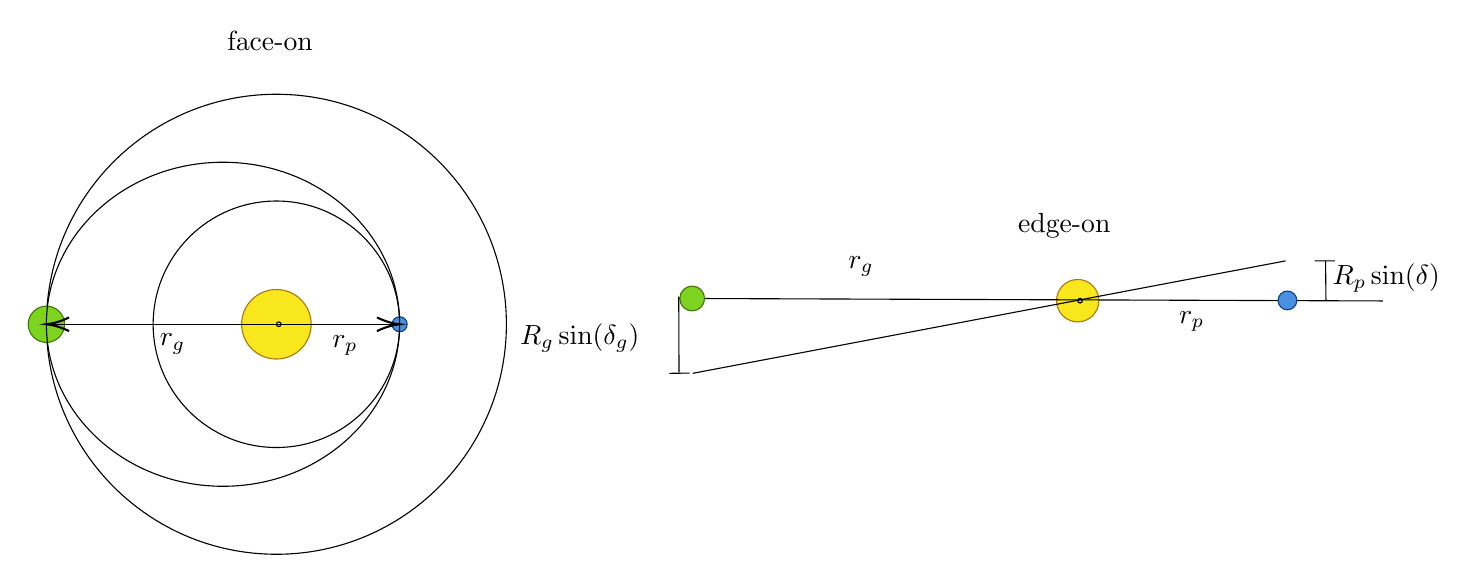
\begin{tikzpicture}[x=0.75pt,y=0.75pt,yscale=-1,xscale=1]
			%uncomment if require: \path (0,436); %set diagram left start at 0, and has height of 436
			
			%Shape: Circle [id:dp03596179299315061] 
			\draw  [color={rgb, 255:red, 171; green, 119; blue, 16 }  ,draw opacity=1 ][fill={rgb, 255:red, 248; green, 231; blue, 28 }  ,fill opacity=1 ] (104.13,242.63) .. controls (104.13,233.37) and (111.62,225.88) .. (120.88,225.88) .. controls (130.13,225.88) and (137.63,233.37) .. (137.63,242.63) .. controls (137.63,251.88) and (130.13,259.38) .. (120.88,259.38) .. controls (111.62,259.38) and (104.13,251.88) .. (104.13,242.63) -- cycle ;
			%Shape: Circle [id:dp1708405127229844] 
			\draw   (61.5,242.63) .. controls (61.5,209.83) and (88.08,183.25) .. (120.88,183.25) .. controls (153.67,183.25) and (180.25,209.83) .. (180.25,242.63) .. controls (180.25,275.42) and (153.67,302) .. (120.88,302) .. controls (88.08,302) and (61.5,275.42) .. (61.5,242.63) -- cycle ;
			%Shape: Circle [id:dp8549680049893815] 
			\draw   (10.06,242.63) .. controls (10.06,181.42) and (59.67,131.81) .. (120.88,131.81) .. controls (182.08,131.81) and (231.69,181.42) .. (231.69,242.63) .. controls (231.69,303.83) and (182.08,353.44) .. (120.88,353.44) .. controls (59.67,353.44) and (10.06,303.83) .. (10.06,242.63) -- cycle ;
			%Shape: Circle [id:dp2793501385943771] 
			\draw  [color={rgb, 255:red, 8; green, 65; blue, 132 }  ,draw opacity=1 ][fill={rgb, 255:red, 74; green, 144; blue, 226 }  ,fill opacity=1 ] (176.63,242.63) .. controls (176.63,240.62) and (178.25,239) .. (180.25,239) .. controls (182.25,239) and (183.88,240.62) .. (183.88,242.63) .. controls (183.88,244.63) and (182.25,246.25) .. (180.25,246.25) .. controls (178.25,246.25) and (176.63,244.63) .. (176.63,242.63) -- cycle ;
			%Shape: Circle [id:dp9038581046929319] 
			\draw  [color={rgb, 255:red, 65; green, 117; blue, 5 }  ,draw opacity=1 ][fill={rgb, 255:red, 126; green, 211; blue, 33 }  ,fill opacity=1 ] (1.31,242.63) .. controls (1.31,237.79) and (5.23,233.88) .. (10.06,233.88) .. controls (14.89,233.88) and (18.81,237.79) .. (18.81,242.63) .. controls (18.81,247.46) and (14.89,251.38) .. (10.06,251.38) .. controls (5.23,251.38) and (1.31,247.46) .. (1.31,242.63) -- cycle ;
			%Shape: Ellipse [id:dp7630996374005055] 
			\draw   (10.06,242.63) .. controls (10.06,199.51) and (48.16,164.56) .. (95.16,164.56) .. controls (142.15,164.56) and (180.25,199.51) .. (180.25,242.63) .. controls (180.25,285.74) and (142.15,320.69) .. (95.16,320.69) .. controls (48.16,320.69) and (10.06,285.74) .. (10.06,242.63) -- cycle ;
			%Straight Lines [id:da5475915682132575] 
			\draw    (120.88,242.63) -- (178.25,242.63) ;
			\draw [shift={(180.25,242.63)}, rotate = 180] [color={rgb, 255:red, 0; green, 0; blue, 0 }  ][line width=0.75]    (10.93,-3.29) .. controls (6.95,-1.4) and (3.31,-0.3) .. (0,0) .. controls (3.31,0.3) and (6.95,1.4) .. (10.93,3.29)   ;
			%Straight Lines [id:da17116842678457278] 
			\draw    (120.88,242.63) -- (12.06,242.63) ;
			\draw [shift={(10.06,242.63)}, rotate = 360] [color={rgb, 255:red, 0; green, 0; blue, 0 }  ][line width=0.75]    (10.93,-3.29) .. controls (6.95,-1.4) and (3.31,-0.3) .. (0,0) .. controls (3.31,0.3) and (6.95,1.4) .. (10.93,3.29)   ;
			%Shape: Circle [id:dp20334584839538872] 
			\draw   (120.88,242.63) .. controls (120.88,242) and (121.38,241.5) .. (122,241.5) .. controls (122.62,241.5) and (123.13,242) .. (123.13,242.63) .. controls (123.13,243.25) and (122.62,243.75) .. (122,243.75) .. controls (121.38,243.75) and (120.88,243.25) .. (120.88,242.63) -- cycle ;
			%Shape: Ellipse [id:dp19798246142154774] 
			\draw  [color={rgb, 255:red, 171; green, 119; blue, 16 }  ,draw opacity=1 ][fill={rgb, 255:red, 248; green, 231; blue, 28 }  ,fill opacity=1 ] (496.75,231.26) .. controls (496.75,225.62) and (501.32,221.04) .. (506.95,221.04) .. controls (512.58,221.04) and (517.15,225.62) .. (517.15,231.26) .. controls (517.15,236.91) and (512.58,241.49) .. (506.95,241.49) .. controls (501.32,241.49) and (496.75,236.91) .. (496.75,231.26) -- cycle ;
			%Straight Lines [id:da42389087296452166] 
			\draw    (321.2,230.21) -- (654,231.4) ;
			%Shape: Ellipse [id:dp4081848662496641] 
			\draw  [color={rgb, 255:red, 8; green, 65; blue, 132 }  ,draw opacity=1 ][fill={rgb, 255:red, 74; green, 144; blue, 226 }  ,fill opacity=1 ] (603.49,231.15) .. controls (603.49,228.65) and (605.5,226.63) .. (607.99,226.63) .. controls (610.48,226.63) and (612.5,228.65) .. (612.5,231.15) .. controls (612.5,233.64) and (610.48,235.67) .. (607.99,235.67) .. controls (605.5,235.67) and (603.49,233.64) .. (603.49,231.15) -- cycle ;
			%Shape: Ellipse [id:dp6308665591196385] 
			\draw  [color={rgb, 255:red, 65; green, 117; blue, 5 }  ,draw opacity=1 ][fill={rgb, 255:red, 126; green, 211; blue, 33 }  ,fill opacity=1 ] (315.23,230.21) .. controls (315.23,226.9) and (317.91,224.23) .. (321.2,224.23) .. controls (324.5,224.23) and (327.17,226.9) .. (327.17,230.21) .. controls (327.17,233.51) and (324.5,236.19) .. (321.2,236.19) .. controls (317.91,236.19) and (315.23,233.51) .. (315.23,230.21) -- cycle ;
			%Straight Lines [id:da09309059887901783] 
			\draw    (321.45,266.27) -- (607.09,212.09) ;
			%Shape: Circle [id:dp03761874052377334] 
			\draw   (506.95,231.26) .. controls (506.95,230.64) and (507.45,230.14) .. (508.08,230.14) .. controls (508.7,230.14) and (509.2,230.64) .. (509.2,231.26) .. controls (509.2,231.89) and (508.7,232.39) .. (508.08,232.39) .. controls (507.45,232.39) and (506.95,231.89) .. (506.95,231.26) -- cycle ;
			%Straight Lines [id:da5130005342535828] 
			\draw    (621.09,212.09) -- (630.82,212.07) ;
			%Straight Lines [id:da37471795216790005] 
			\draw    (626.36,212.09) -- (626.55,231) ;
			%Straight Lines [id:da6690627214782825] 
			\draw    (319.96,266.15) -- (310.23,266.27) ;
			%Straight Lines [id:da943260883611647] 
			\draw    (314.85,265.78) -- (314.73,229.36) ;
			
			% Text Node
			\draw (63.5,246.03) node [anchor=north west][inner sep=0.75pt]    {$r_{g}$};
			% Text Node
			\draw (554.5,235.08) node [anchor=north west][inner sep=0.75pt]    {$r_{p}$};
			% Text Node
			\draw (628.45,212.26) node [anchor=north west][inner sep=0.75pt]    {$R_{p}\sin( \delta )$};
			% Text Node
			\draw (146.64,246.63) node [anchor=north west][inner sep=0.75pt]    {$r_{p}$};
			% Text Node
			\draw (395.18,208.71) node [anchor=north west][inner sep=0.75pt]    {$r_{g}$};
			% Text Node
			\draw (237.09,240.95) node [anchor=north west][inner sep=0.75pt]    {$R_{g}\sin( \delta _{g})$};
			% Text Node
			\draw (477,188) node [anchor=north west][inner sep=0.75pt]   [align=left] {{\fontfamily{helvet}\selectfont \textit{edge-on}}};
			% Text Node
			\draw (96,100) node [anchor=north west][inner sep=0.75pt]   [align=left] {{\fontfamily{helvet}\selectfont \textit{face-on}}};
			
			
		\end{tikzpicture}
	
\caption{Representation of the inclination of the transfer orbit. In the \emph{edge-on} figure, the planets were shown smaller than the departure and arrival lines intentionally to facilitate the visualization of distances.}
\end{figure}

By triangle similarity, we can relate the data:

$$\frac{R_p \sin{(\delta)}}{r_p} = \frac{R_g \sin{(\delta_g)}}{r_g}$$

Therefore:

$$\delta_g = \arcsin{\left( \frac{R_p r_g}{R_g r_p} \sin{(\delta)} \right)}$$

Substituting the values, we find $\delta_g = -11^\circ 57'$. Note that we changed the latitude value to negative, which becomes clear from the figure.

\ut{E.3} Consider that at the moment of launch, Plutão II was at angular position $0^\circ$. Upon arriving at Genibals, Plutão II will be in a different position and Genibals will be at position $180^\circ$. To know the position of Plutão II, we just need to relate the travel time of the outbound trip to the planet's period.

By Kepler's third law, $T \propto a^{3/2}$. The semi-major axis of the transfer orbit is $a = \frac{r_p + r_g}{2}$, so:

$$T_{transfer} = T_p \left( \frac{r_p + r_g}{2 r_p} \right)^{3/2}$$

However, the outbound travel time is only half of the total period of the transfer orbit, thus: $T_{outbound} = 0.63 T_p$. This means that Plutão II traveled an angular distance of $\Delta \phi = 0.63 \cdot 360^\circ$. Therefore, the angle $\theta$ in the figure below is $\theta_1 = 46.8^\circ$.

	\begin{figure}[htpb]
		\centering
		
		\tikzset{every picture/.style={line width=0.75pt}} %set default line width to 0.75pt        
		
		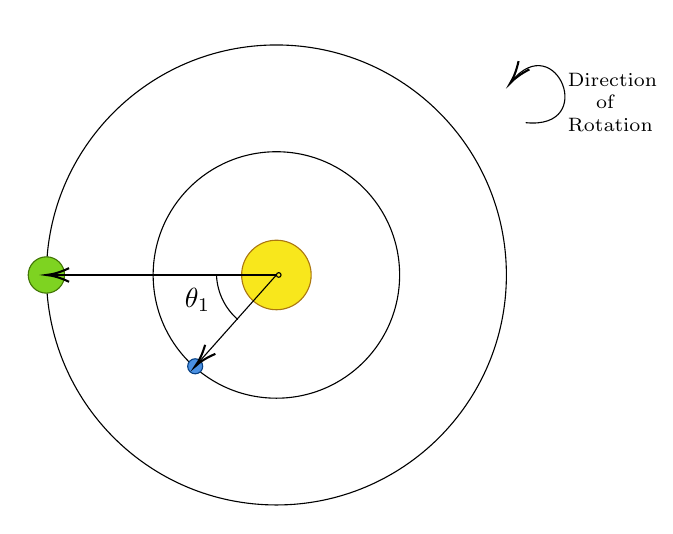
\begin{tikzpicture}[x=0.75pt,y=0.75pt,yscale=-1,xscale=1]
			%uncomment if require: \path (0,436); %set diagram left start at 0, and has height of 436
			
			%Shape: Circle [id:dp49050764243391964] 
			\draw  [color={rgb, 255:red, 171; green, 119; blue, 16 }  ,draw opacity=1 ][fill={rgb, 255:red, 248; green, 231; blue, 28 }  ,fill opacity=1 ] (104.13,242.63) .. controls (104.13,233.37) and (111.62,225.88) .. (120.88,225.88) .. controls (130.13,225.88) and (137.63,233.37) .. (137.63,242.63) .. controls (137.63,251.88) and (130.13,259.38) .. (120.88,259.38) .. controls (111.62,259.38) and (104.13,251.88) .. (104.13,242.63) -- cycle ;
			%Shape: Circle [id:dp3934909707274261] 
			\draw   (61.5,242.63) .. controls (61.5,209.83) and (88.08,183.25) .. (120.88,183.25) .. controls (153.67,183.25) and (180.25,209.83) .. (180.25,242.63) .. controls (180.25,275.42) and (153.67,302) .. (120.88,302) .. controls (88.08,302) and (61.5,275.42) .. (61.5,242.63) -- cycle ;
			%Shape: Circle [id:dp2535797775502542] 
			\draw   (10.06,242.63) .. controls (10.06,181.42) and (59.67,131.81) .. (120.88,131.81) .. controls (182.08,131.81) and (231.69,181.42) .. (231.69,242.63) .. controls (231.69,303.83) and (182.08,353.44) .. (120.88,353.44) .. controls (59.67,353.44) and (10.06,303.83) .. (10.06,242.63) -- cycle ;
			%Shape: Circle [id:dp3725253916573583] 
			\draw  [color={rgb, 255:red, 8; green, 65; blue, 132 }  ,draw opacity=1 ][fill={rgb, 255:red, 74; green, 144; blue, 226 }  ,fill opacity=1 ] (78.13,286.63) .. controls (78.13,284.62) and (79.75,283) .. (81.75,283) .. controls (83.75,283) and (85.38,284.62) .. (85.38,286.63) .. controls (85.38,288.63) and (83.75,290.25) .. (81.75,290.25) .. controls (79.75,290.25) and (78.13,288.63) .. (78.13,286.63) -- cycle ;
			%Shape: Circle [id:dp7411305466921247] 
			\draw  [color={rgb, 255:red, 65; green, 117; blue, 5 }  ,draw opacity=1 ][fill={rgb, 255:red, 126; green, 211; blue, 33 }  ,fill opacity=1 ] (1.31,242.63) .. controls (1.31,237.79) and (5.23,233.88) .. (10.06,233.88) .. controls (14.89,233.88) and (18.81,237.79) .. (18.81,242.63) .. controls (18.81,247.46) and (14.89,251.38) .. (10.06,251.38) .. controls (5.23,251.38) and (1.31,247.46) .. (1.31,242.63) -- cycle ;
			%Straight Lines [id:da47905217294623736] 
			\draw    (120.88,242.63) -- (83.08,285.13) ;
			\draw [shift={(81.75,286.63)}, rotate = 311.64] [color={rgb, 255:red, 0; green, 0; blue, 0 }  ][line width=0.75]    (10.93,-3.29) .. controls (6.95,-1.4) and (3.31,-0.3) .. (0,0) .. controls (3.31,0.3) and (6.95,1.4) .. (10.93,3.29)   ;
			%Straight Lines [id:da08662751708334238] 
			\draw    (120.88,242.63) -- (12.06,242.63) ;
			\draw [shift={(10.06,242.63)}, rotate = 360] [color={rgb, 255:red, 0; green, 0; blue, 0 }  ][line width=0.75]    (10.93,-3.29) .. controls (6.95,-1.4) and (3.31,-0.3) .. (0,0) .. controls (3.31,0.3) and (6.95,1.4) .. (10.93,3.29)   ;
			%Shape: Circle [id:dp993746110660156] 
			\draw   (120.88,242.63) .. controls (120.88,242) and (121.38,241.5) .. (122,241.5) .. controls (122.62,241.5) and (123.13,242) .. (123.13,242.63) .. controls (123.13,243.25) and (122.62,243.75) .. (122,243.75) .. controls (121.38,243.75) and (120.88,243.25) .. (120.88,242.63) -- cycle ;
			%Shape: Arc [id:dp9480557108989549] 
			\draw  [draw opacity=0] (102.27,264.1) .. controls (96.36,258.94) and (92.49,251.49) .. (92.04,243.13) -- (122,241.5) -- cycle ; \draw   (102.27,264.1) .. controls (96.36,258.94) and (92.49,251.49) .. (92.04,243.13) ;
			%Curve Lines [id:da9356433285441141] 
			\draw    (241,169.25) .. controls (275.97,172.7) and (255.63,123.75) .. (234.47,149.04) ;
			\draw [shift={(233.5,150.25)}, rotate = 307.52] [color={rgb, 255:red, 0; green, 0; blue, 0 }  ][line width=0.75]    (10.93,-3.29) .. controls (6.95,-1.4) and (3.31,-0.3) .. (0,0) .. controls (3.31,0.3) and (6.95,1.4) .. (10.93,3.29)   ;
			
			% Text Node
			\draw (75.5,247.9) node [anchor=north west][inner sep=0.75pt]    {$\theta _{1}$};
			% Text Node
			\draw (260,140) node [anchor=north west][inner sep=0.75pt]  [font=\scriptsize] [align=left] {\begin{minipage}[lt]{26.95pt}\setlength\topsep{0pt}
					\begin{center}
						{\fontfamily{helvet}\selectfont Direction of}\\{\fontfamily{helvet}\selectfont Rotation}
					\end{center}
					
			\end{minipage}};
			
			
		\end{tikzpicture}
	
\caption{Representation of the orbital configuration and determination of the direction of rotation of the planets around the star}
\end{figure}

Note that during the course of a one-way trip, Plutão II travels an angle of $\Delta \phi = 180^\circ + \theta_1$. Therefore, for the spacecraft to reach the planet, it must be launched when Plutão II is half a revolution plus $\theta_1$ degrees before the landing position. The landing position is always half a revolution ahead of Genibals, so the orbital configuration at the time of launch for the return trip must be:

	\begin{figure}[htpb]
		\centering
		
		\tikzset{every picture/.style={line width=0.75pt}} %set default line width to 0.75pt        
		
		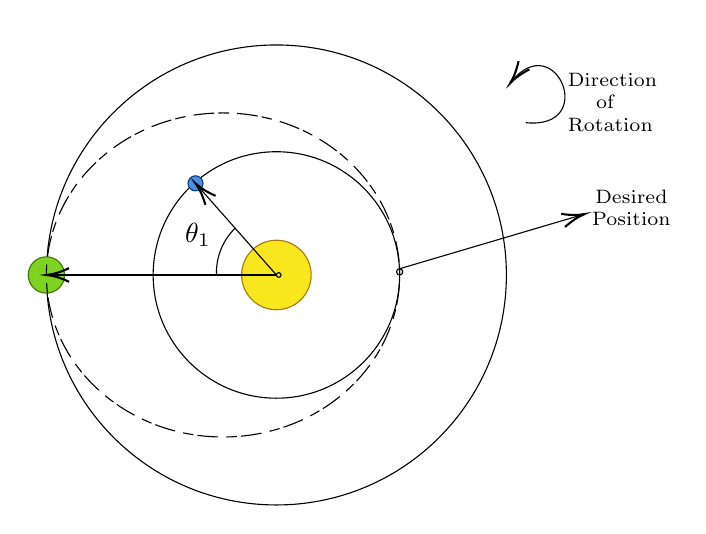
\begin{tikzpicture}[x=0.75pt,y=0.75pt,yscale=-1,xscale=1]
			%uncomment if require: \path (0,436); %set diagram left start at 0, and has height of 436
			
			%Shape: Circle [id:dp49050764243391964] 
			\draw  [color={rgb, 255:red, 171; green, 119; blue, 16 }  ,draw opacity=1 ][fill={rgb, 255:red, 248; green, 231; blue, 28 }  ,fill opacity=1 ] (104.13,242.63) .. controls (104.13,233.37) and (111.62,225.88) .. (120.88,225.88) .. controls (130.13,225.88) and (137.63,233.37) .. (137.63,242.63) .. controls (137.63,251.88) and (130.13,259.38) .. (120.88,259.38) .. controls (111.62,259.38) and (104.13,251.88) .. (104.13,242.63) -- cycle ;
			%Shape: Circle [id:dp3934909707274261] 
			\draw   (61.5,242.63) .. controls (61.5,209.83) and (88.08,183.25) .. (120.88,183.25) .. controls (153.67,183.25) and (180.25,209.83) .. (180.25,242.63) .. controls (180.25,275.42) and (153.67,302) .. (120.88,302) .. controls (88.08,302) and (61.5,275.42) .. (61.5,242.63) -- cycle ;
			%Shape: Circle [id:dp2535797775502542] 
			\draw   (10.06,242.63) .. controls (10.06,181.42) and (59.67,131.81) .. (120.88,131.81) .. controls (182.08,131.81) and (231.69,181.42) .. (231.69,242.63) .. controls (231.69,303.83) and (182.08,353.44) .. (120.88,353.44) .. controls (59.67,353.44) and (10.06,303.83) .. (10.06,242.63) -- cycle ;
			%Shape: Circle [id:dp3725253916573583] 
			\draw  [color={rgb, 255:red, 8; green, 65; blue, 132 }  ,draw opacity=1 ][fill={rgb, 255:red, 74; green, 144; blue, 226 }  ,fill opacity=1 ] (78.28,198.48) .. controls (78.28,196.48) and (79.91,194.85) .. (81.91,194.85) .. controls (83.91,194.85) and (85.53,196.48) .. (85.53,198.48) .. controls (85.53,200.48) and (83.91,202.1) .. (81.91,202.1) .. controls (79.91,202.1) and (78.28,200.48) .. (78.28,198.48) -- cycle ;
			%Shape: Circle [id:dp7411305466921247] 
			\draw  [color={rgb, 255:red, 65; green, 117; blue, 5 }  ,draw opacity=1 ][fill={rgb, 255:red, 126; green, 211; blue, 33 }  ,fill opacity=1 ] (1.31,242.63) .. controls (1.31,237.79) and (5.23,233.88) .. (10.06,233.88) .. controls (14.89,233.88) and (18.81,237.79) .. (18.81,242.63) .. controls (18.81,247.46) and (14.89,251.38) .. (10.06,251.38) .. controls (5.23,251.38) and (1.31,247.46) .. (1.31,242.63) -- cycle ;
			%Straight Lines [id:da47905217294623736] 
			\draw    (120.88,242.63) -- (83.23,199.98) ;
			\draw [shift={(81.91,198.48)}, rotate = 48.57] [color={rgb, 255:red, 0; green, 0; blue, 0 }  ][line width=0.75]    (10.93,-3.29) .. controls (6.95,-1.4) and (3.31,-0.3) .. (0,0) .. controls (3.31,0.3) and (6.95,1.4) .. (10.93,3.29)   ;
			%Straight Lines [id:da08662751708334238] 
			\draw    (120.88,242.63) -- (12.06,242.63) ;
			\draw [shift={(10.06,242.63)}, rotate = 360] [color={rgb, 255:red, 0; green, 0; blue, 0 }  ][line width=0.75]    (10.93,-3.29) .. controls (6.95,-1.4) and (3.31,-0.3) .. (0,0) .. controls (3.31,0.3) and (6.95,1.4) .. (10.93,3.29)   ;
			%Shape: Circle [id:dp993746110660156] 
			\draw   (120.88,242.63) .. controls (120.88,242) and (121.38,241.5) .. (122,241.5) .. controls (122.62,241.5) and (123.13,242) .. (123.13,242.63) .. controls (123.13,243.25) and (122.62,243.75) .. (122,243.75) .. controls (121.38,243.75) and (120.88,243.25) .. (120.88,242.63) -- cycle ;
			%Shape: Arc [id:dp9480557108989549] 
			\draw  [draw opacity=0] (92.01,242.16) .. controls (92,241.94) and (92,241.72) .. (92,241.5) .. controls (92,233.04) and (95.5,225.39) .. (101.14,219.94) -- (122,241.5) -- cycle ; \draw   (92.01,242.16) .. controls (92,241.94) and (92,241.72) .. (92,241.5) .. controls (92,233.04) and (95.5,225.39) .. (101.14,219.94) ;
			%Curve Lines [id:da9356433285441141] 
			\draw    (241,169.25) .. controls (275.97,172.7) and (255.63,123.75) .. (234.47,149.04) ;
			\draw [shift={(233.5,150.25)}, rotate = 307.52] [color={rgb, 255:red, 0; green, 0; blue, 0 }  ][line width=0.75]    (10.93,-3.29) .. controls (6.95,-1.4) and (3.31,-0.3) .. (0,0) .. controls (3.31,0.3) and (6.95,1.4) .. (10.93,3.29)   ;
			%Shape: Ellipse [id:dp26738677711207925] 
			\draw  [dash pattern={on 3.75pt off 3pt on 7.5pt off 1.5pt}] (10.06,242.63) .. controls (10.06,199.51) and (48.16,164.56) .. (95.16,164.56) .. controls (142.15,164.56) and (180.25,199.51) .. (180.25,242.63) .. controls (180.25,285.74) and (142.15,320.69) .. (95.16,320.69) .. controls (48.16,320.69) and (10.06,285.74) .. (10.06,242.63) -- cycle ;
			%Shape: Circle [id:dp03927003784283323] 
			\draw   (178.75,241.13) .. controls (178.75,240.3) and (179.42,239.63) .. (180.25,239.63) .. controls (181.08,239.63) and (181.75,240.3) .. (181.75,241.13) .. controls (181.75,241.95) and (181.08,242.63) .. (180.25,242.63) .. controls (179.42,242.63) and (178.75,241.95) .. (178.75,241.13) -- cycle ;
			%Straight Lines [id:da4230491453650722] 
			\draw    (180.25,239.63) -- (267.58,213.82) ;
			\draw [shift={(269.5,213.25)}, rotate = 163.54] [color={rgb, 255:red, 0; green, 0; blue, 0 }  ][line width=0.75]    (10.93,-3.29) .. controls (6.95,-1.4) and (3.31,-0.3) .. (0,0) .. controls (3.31,0.3) and (6.95,1.4) .. (10.93,3.29)   ;
			
			% Text Node
			\draw (75.68,216.26) node [anchor=north west][inner sep=0.75pt]    {$\theta _{1}$};
			% Text Node
			\draw (260,140) node [anchor=north west][inner sep=0.75pt]  [font=\scriptsize] [align=left] {\begin{minipage}[lt]{26.95pt}\setlength\topsep{0pt}
					\begin{center}
						{\fontfamily{helvet}\selectfont Direction of}\\{\fontfamily{helvet}\selectfont Rotation}
					\end{center}
					
			\end{minipage}};
			% Text Node
			\draw (269.5,200.5) node [anchor=north west][inner sep=0.75pt]  [font=\scriptsize] [align=left] {\begin{minipage}[lt]{31.71pt}\setlength\topsep{0pt}
					\begin{center}
						Desired\\Position
					\end{center}
					
			\end{minipage}};
			
			
		\end{tikzpicture}
	
\caption{Geometry of the transfer curve and prediction of arrival position}
\end{figure}

Note that the new angle, measured in the direction of rotation, between the planets is $\theta_2 = 360^\circ - \theta_1$. So the next question is: how much time must pass for the angle between the planets to increase to $\theta_2$? From the angular velocity of each planet we have:

$$\frac{360^\circ}{T_p}\Delta t - \frac{360^\circ}{T_g}\Delta t = \Delta \theta = 360^\circ - 2\theta_1$$

Substituting the values we find:

$$\Delta t = 2.11 T_p = 2.11 \text{ Plutonian years}$$

\ut{E.4} For this, we must calculate the $\Delta v$ required for each maneuver.

\begin{enumerate}

\item $\Delta v_1$

For the first maneuver, we must not only escape the gravitational field of Plutão II but also increase the spacecraft's velocity to enter the transfer orbit. From the launch location, the tangential velocity is $v_t = \dfrac{2\pi R_p \cos{(\delta)}}{t_p}$:

\begin{figure}[htpb]
    \centering
    \includegraphics[scale = 0.7]{images/imageee.png}
    \caption{Launch latitude and radius of the circle of points with the same latitude}
\end{figure}

Since the planet rotates in the same direction as its orbit, this velocity aids the launch. To escape the planet, the total spacecraft speed must be $v = \sqrt{\dfrac{2GM_p}{R_p}}$, therefore $\Delta v_1' = \sqrt{\dfrac{2GM_p}{R_p}} - \dfrac{2\pi R_p \cos{(\delta)}}{t_p} = 11.145\text{ km/s}$. After this velocity change, the craft leaves Plutão II's gravitational influence and, relative to Scorp, moves with the same orbital velocity as Plutão II\footnote{This occurs because the rocket ends at rest relative to Plutão II}. This means another $\Delta v_1''$ is required:

$$\Delta v_1'' = \sqrt{GM_s\left(\frac{2}{r_p} - \frac{1}{a}\right)} - \sqrt{\frac{GM_s}{r_p}}$$

$$\Delta v_1'' = \sqrt{\frac{2GM_s r_g}{r_p (r_p + r_g)}} - \sqrt{\frac{GM_s}{r_p}}$$

Substituting the values: $\Delta v_1'' = 2.061\text{ km/s}$. Therefore, $\Delta v_1 = 13.206\text{ km/s}$.

\item $\Delta v_2$

To leave the transfer orbit and enter Genibals' orbit:

$$\Delta v_2' = \sqrt{\frac{GM_s}{r_g}} - \sqrt{\frac{2GM_s r_p}{r_g (r_p + r_g)}} = 1.918\text{ km/s}$$

\item $\Delta v_3$

When the spacecraft reaches the planet, after performing $\Delta v_2$, it would have a speed $v = \sqrt{\dfrac{2GM_g}{R_g}}$. However, it must arrive with a speed $v' = \dfrac{2\pi R_g \cos{\delta_g}}{t_g}$ for a perfect landing (due to the planet's rotation), so $|\Delta v_3| = \sqrt{\dfrac{2GM_g}{R_g}} - \dfrac{2\pi R_g \cos{\delta_g}}{t_g} = 29.704\text{ km/s}$.

\item $\Delta v_4$

For $\Delta v_4$, we simply undo $\Delta v_3$ to leave Genibals: $\Delta v_4 = \Delta v_3 = 29.704 \text{ km/s}$.

\item $\Delta v_5$

For $\Delta v_5$, we undo $\Delta v_2$ to enter the transfer orbit: $\Delta v_5 = \Delta v_2 = 1.918 \text{ km/s}$.

\item $\Delta v_6$

To enter Plutão II's orbit, the rocket must reduce its velocity:

$$|\Delta v_6| = \sqrt{\frac{2GM_s r_g}{r_p (r_p + r_g)}} - \sqrt{\frac{GM_s}{r_p}} = 2.061 \text{ km/s}$$

\item $\Delta v_7$

The rocket reaches the planet's surface at $v = \sqrt{\dfrac{2GM_p}{R_p}}$, but for a safe landing, it must have $v' = \dfrac{2\pi R_p \cos{(\delta)}}{t_p}$, so we apply $|\Delta v_7| = \sqrt{\dfrac{2GM_p}{R_p}} - \dfrac{2\pi R_p \cos{(\delta)}}{t_p} = 11.145\text{ km/s}$.

\end{enumerate}

Now that we have all $\Delta v$ values, we need to find the corresponding mass changes to determine the total mass. To achieve a given $\Delta v$, a certain amount of fluid and its container must be ejected; thus, there are two propulsions, with the fluid propulsion obeying the relation $\Delta v' = u \ln{\left( \dfrac{m_0}{m_F} \right)}$.

First, we find a relation between the fluid mass and container mass. The fluid mass is $m_f = \pi(2-0.1)^2 h \rho$ (considering the container thickness), while the container mass is $m_c = \pi(2^2 - 1.9^2) h \rho'$. Note that $\dfrac{m_c}{m_f} = \dfrac{0.39(4.01)}{3.61(1.3)}$, meaning $m_c \approx \dfrac{1}{3} m_f$.

$$\Delta v = \Delta v_f + \Delta v_c$$

$$\Delta v_f = u \ln{\left(\frac{m_0}{m_0 - m_f}\right)}$$

For $\Delta v_c$, we must consider linear momentum conservation:

	\begin{figure}[htpb]
		\centering
		
		\tikzset{every picture/.style={line width=0.75pt}} %set default line width to 0.75pt        
		
		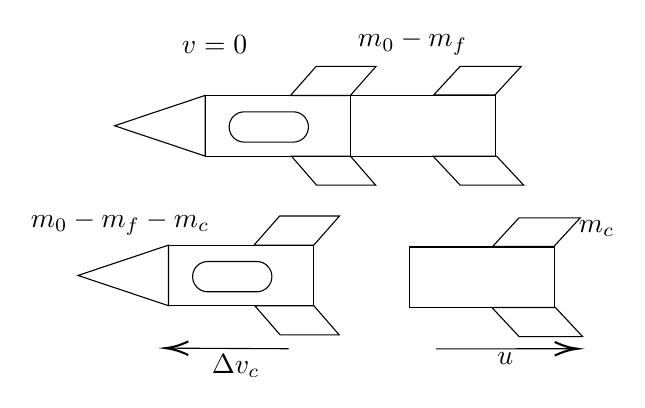
\begin{tikzpicture}[x=0.75pt,y=0.75pt,yscale=-1,xscale=1]
			%uncomment if require: \path (0,436); %set diagram left start at 0, and has height of 436
			
			%Shape: Rectangle [id:dp28716406868861344] 
			\draw   (170,131.22) -- (240,131.22) -- (240,160.42) -- (170,160.42) -- cycle ;
			%Shape: Rectangle [id:dp928536430364594] 
			\draw   (100,131.22) -- (170,131.22) -- (170,160.42) -- (100,160.42) -- cycle ;
			%Flowchart: Extract [id:dp6198971966656859] 
			\draw   (56.4,145.82) -- (100,131.22) -- (100,160.42) -- cycle ;
			%Shape: Parallelogram [id:dp2731040142473209] 
			\draw   (153.52,117.21) -- (182.36,117.21) -- (170,131.22) -- (141.16,131.22) -- cycle ;
			%Shape: Parallelogram [id:dp5244106130770332] 
			\draw   (222.85,117.21) -- (252.36,117.21) -- (239.71,130.93) -- (210.2,130.93) -- cycle ;
			%Shape: Parallelogram [id:dp5473813893829482] 
			\draw   (240.4,160.42) -- (209.8,160.42) -- (222.91,174.43) -- (253.51,174.43) -- cycle ;
			%Shape: Parallelogram [id:dp5581751213406347] 
			\draw   (170,160.42) -- (141.55,160.42) -- (153.74,174.43) -- (182.19,174.43) -- cycle ;
			%Rounded Rect [id:dp5232087385928359] 
			\draw   (111.6,146.4) .. controls (111.6,142.37) and (114.87,139.1) .. (118.9,139.1) -- (142.5,139.1) .. controls (146.53,139.1) and (149.8,142.37) .. (149.8,146.4) -- (149.8,146.4) .. controls (149.8,150.43) and (146.53,153.7) .. (142.5,153.7) -- (118.9,153.7) .. controls (114.87,153.7) and (111.6,150.43) .. (111.6,146.4) -- cycle ;
			%Shape: Rectangle [id:dp8857065612329185] 
			\draw   (198.4,204.21) -- (268.4,204.21) -- (268.4,233.4) -- (198.4,233.4) -- cycle ;
			%Shape: Rectangle [id:dp9685608723610961] 
			\draw   (82.4,203.33) -- (152.4,203.33) -- (152.4,232.53) -- (82.4,232.53) -- cycle ;
			%Flowchart: Extract [id:dp8224636054415246] 
			\draw   (38.8,217.93) -- (82.4,203.33) -- (82.4,232.53) -- cycle ;
			%Shape: Parallelogram [id:dp8127195785947527] 
			\draw   (135.92,189.32) -- (164.76,189.32) -- (152.4,203.33) -- (123.56,203.33) -- cycle ;
			%Shape: Parallelogram [id:dp41281907780667204] 
			\draw   (251.25,190.19) -- (280.76,190.19) -- (268.11,203.92) -- (238.6,203.92) -- cycle ;
			%Shape: Parallelogram [id:dp31666730749138683] 
			\draw   (268.8,233.4) -- (238.2,233.4) -- (251.31,247.41) -- (281.91,247.41) -- cycle ;
			%Shape: Parallelogram [id:dp26773518147422015] 
			\draw   (152.4,232.53) -- (123.95,232.53) -- (136.14,246.54) -- (164.59,246.54) -- cycle ;
			%Rounded Rect [id:dp22540702493118414] 
			\draw   (94,218.51) .. controls (94,214.48) and (97.27,211.21) .. (101.3,211.21) -- (124.9,211.21) .. controls (128.93,211.21) and (132.2,214.48) .. (132.2,218.51) -- (132.2,218.51) .. controls (132.2,222.54) and (128.93,225.81) .. (124.9,225.81) -- (101.3,225.81) .. controls (97.27,225.81) and (94,222.54) .. (94,218.51) -- cycle ;
			%Straight Lines [id:da8853264423863085] 
			\draw    (140.2,253.25) -- (83,252.97) ;
			\draw [shift={(81,252.96)}, rotate = 0.28] [color={rgb, 255:red, 0; green, 0; blue, 0 }  ][line width=0.75]    (10.93,-3.29) .. controls (6.95,-1.4) and (3.31,-0.3) .. (0,0) .. controls (3.31,0.3) and (6.95,1.4) .. (10.93,3.29)   ;
			%Straight Lines [id:da4718880738596367] 
			\draw    (211.2,253.31) -- (277.4,253.26) ;
			\draw [shift={(279.4,253.25)}, rotate = 179.95] [color={rgb, 255:red, 0; green, 0; blue, 0 }  ][line width=0.75]    (10.93,-3.29) .. controls (6.95,-1.4) and (3.31,-0.3) .. (0,0) .. controls (3.31,0.3) and (6.95,1.4) .. (10.93,3.29)   ;
			
			% Text Node
			\draw (87.6,101) node [anchor=north west][inner sep=0.75pt]    {$v=0$};
			% Text Node
			\draw (102,254.87) node [anchor=north west][inner sep=0.75pt]    {$\Delta v_{c}$};
			% Text Node
			\draw (239.6,253.97) node [anchor=north west][inner sep=0.75pt]    {$u$};
			% Text Node
			\draw (172.4,98.83) node [anchor=north west][inner sep=0.75pt]    {$m_{0} -m_{f}$};
			% Text Node
			\draw (14.8,185.68) node [anchor=north west][inner sep=0.75pt]    {$m_{0} -m_{f} -m_{c}$};
			% Text Node
			\draw (278.8,190.35) node [anchor=north west][inner sep=0.75pt]    {$m_{c}$};
			
			
		\end{tikzpicture}
		
	
\caption{Representation of stage change and release of rocket modules to achieve thrust}
\end{figure}

$$(m_0 - m_f - m_c)\Delta v_c = m_c u$$

However, we want to express the mass factors only in terms of the final mass $m_F$ and the initial mass $m_0$ for the maneuver: $m_F = m_0 - m_c - m_f = m_0 - \dfrac{4}{3} m_f$. Therefore, $m_c = \dfrac{m_0 - m_F}{4}$ and $m_f = \dfrac{3(m_0 - m_F)}{4}$.

$$\Delta v = u \ln{\left(\frac{4 m_0}{m_0 + 3 m_F}\right)} + u \frac{m_0 - m_F}{4 m_F}$$

Let $x = \dfrac{m_0}{m_F}$:

$$4\frac{\Delta v}{u} = 4 \ln{\left(\frac{4x}{x+3}\right)} + x - 1$$

\begin{equation}
\boxed{\therefore x = 4\frac{\Delta v}{u} + 1 - 4 \ln{\left(\frac{4x}{x+3}\right)}}
\label{k1}
\end{equation}

For the ion engine, we have a similar scheme. Using the ideal gas equation for the gases inside the chamber:

$$V = \frac{nRT}{P} = \frac{m_{ion} RT}{M P}$$

This is the internal volume of the container, so:

$$V = (1.9)^2 \pi \cdot h$$

$$\therefore h = \frac{V}{1.9^2 \pi}$$

The volume of the container material is:

$$V' = \pi (2^2 - 1.9^2) \frac{V}{\pi 1.9^2} = \left( \left( \frac{2}{1.9} \right)^2 - 1 \right) V$$

Therefore, the final expression for the mass of the container in terms of the gas mass is:

$$\therefore m_{chamber} = \rho' \left( \left( \frac{2}{1.9} \right)^2 - 1 \right) \frac{m_{ion} RT}{M P}$$

Substituting the values, we find:

$$m_{chamber} \approx 2 m_{ion}$$

Applying the velocity change equations:

$$\Delta v_1 = v_{ion} \ln\left( \frac{m_0}{m_0 - m_{ion}} \right)$$

And

$$(m_0 - m_{ion} - m_{chamber}) \Delta v_2 = m_{chamber} v_{ion}$$

$$m_F = m_0 - 3 m_{ion} \therefore m_{chamber} = \frac{2}{3} (m_0 - m_F)$$

$$\therefore \Delta v_2 = \frac{2 (m_0 - m_F)}{3 m_F} v_{ion}$$

Adding the velocity increments and letting $x = \dfrac{m_0}{m_F}$:

$$\Delta v = v_{ion} \left( \ln\left( \frac{3x}{2x + 1} \right) + \frac{2}{3} x - \frac{2}{3} \right)$$

\begin{equation}
\boxed{\therefore x = \frac{3 \Delta v}{2 v_{ion}} + 1 - \frac{3}{2} \ln\left( \frac{3x}{2x + 1} \right)}
\label{k2}
\end{equation}

Using equations \ref{k1} and \ref{k2} and iterating the results, we find the following values of $x$:

$$\begin{cases}
x_1 = 9.735\\
x_2 = 1.022\\
x_3 = 25.602\\
x_4 = 25.602\\
x_5 = 1.022\\
x_6 = 1.024\\
x_7 = 7.889\\
\end{cases}$$

Note that $x_i = \dfrac{m_{i-1}}{m_i}$, where $i$ is the $i$-th stage and $m_i$ is the mass after the $i$-th stage. Considering that only the command module lands at the end, we have:

$$x_1 x_2 \dots x_7 = \frac{m_0}{m_1} \frac{m_1}{m_2} \dots \frac{m_6}{m_7} = \frac{m_0}{m_7}$$

Since $m_7$ is the final mass ($m_7 = 10\text{ kg}$):

$$m_0 = 10 \prod_{i=1}^7 x_i \text{ kg}$$

Finally: $m_0 = 538.4$ tons.
	
    \clearpage
    
    
    \fi
\end{document}
